% Options for packages loaded elsewhere
\PassOptionsToPackage{unicode}{hyperref}
\PassOptionsToPackage{hyphens}{url}
%
\documentclass[
  letterpaper,
]{scrbook}

\usepackage{amsmath,amssymb}
\usepackage{lmodern}
\usepackage{iftex}
\ifPDFTeX
  \usepackage[T1]{fontenc}
  \usepackage[utf8]{inputenc}
  \usepackage{textcomp} % provide euro and other symbols
\else % if luatex or xetex
  \usepackage{unicode-math}
  \defaultfontfeatures{Scale=MatchLowercase}
  \defaultfontfeatures[\rmfamily]{Ligatures=TeX,Scale=1}
\fi
% Use upquote if available, for straight quotes in verbatim environments
\IfFileExists{upquote.sty}{\usepackage{upquote}}{}
\IfFileExists{microtype.sty}{% use microtype if available
  \usepackage[]{microtype}
  \UseMicrotypeSet[protrusion]{basicmath} % disable protrusion for tt fonts
}{}
\makeatletter
\@ifundefined{KOMAClassName}{% if non-KOMA class
  \IfFileExists{parskip.sty}{%
    \usepackage{parskip}
  }{% else
    \setlength{\parindent}{0pt}
    \setlength{\parskip}{6pt plus 2pt minus 1pt}}
}{% if KOMA class
  \KOMAoptions{parskip=half}}
\makeatother
\usepackage{xcolor}
\usepackage[left=1in,marginparwidth=2.0666666666667in,textwidth=4.1333333333333in,marginparsep=0.3in]{geometry}
\setlength{\emergencystretch}{3em} % prevent overfull lines
\setcounter{secnumdepth}{5}
% Make \paragraph and \subparagraph free-standing
\ifx\paragraph\undefined\else
  \let\oldparagraph\paragraph
  \renewcommand{\paragraph}[1]{\oldparagraph{#1}\mbox{}}
\fi
\ifx\subparagraph\undefined\else
  \let\oldsubparagraph\subparagraph
  \renewcommand{\subparagraph}[1]{\oldsubparagraph{#1}\mbox{}}
\fi

\usepackage{color}
\usepackage{fancyvrb}
\newcommand{\VerbBar}{|}
\newcommand{\VERB}{\Verb[commandchars=\\\{\}]}
\DefineVerbatimEnvironment{Highlighting}{Verbatim}{commandchars=\\\{\}}
% Add ',fontsize=\small' for more characters per line
\usepackage{framed}
\definecolor{shadecolor}{RGB}{241,243,245}
\newenvironment{Shaded}{\begin{snugshade}}{\end{snugshade}}
\newcommand{\AlertTok}[1]{\textcolor[rgb]{0.68,0.00,0.00}{#1}}
\newcommand{\AnnotationTok}[1]{\textcolor[rgb]{0.37,0.37,0.37}{#1}}
\newcommand{\AttributeTok}[1]{\textcolor[rgb]{0.40,0.45,0.13}{#1}}
\newcommand{\BaseNTok}[1]{\textcolor[rgb]{0.68,0.00,0.00}{#1}}
\newcommand{\BuiltInTok}[1]{\textcolor[rgb]{0.00,0.23,0.31}{#1}}
\newcommand{\CharTok}[1]{\textcolor[rgb]{0.13,0.47,0.30}{#1}}
\newcommand{\CommentTok}[1]{\textcolor[rgb]{0.37,0.37,0.37}{#1}}
\newcommand{\CommentVarTok}[1]{\textcolor[rgb]{0.37,0.37,0.37}{\textit{#1}}}
\newcommand{\ConstantTok}[1]{\textcolor[rgb]{0.56,0.35,0.01}{#1}}
\newcommand{\ControlFlowTok}[1]{\textcolor[rgb]{0.00,0.23,0.31}{#1}}
\newcommand{\DataTypeTok}[1]{\textcolor[rgb]{0.68,0.00,0.00}{#1}}
\newcommand{\DecValTok}[1]{\textcolor[rgb]{0.68,0.00,0.00}{#1}}
\newcommand{\DocumentationTok}[1]{\textcolor[rgb]{0.37,0.37,0.37}{\textit{#1}}}
\newcommand{\ErrorTok}[1]{\textcolor[rgb]{0.68,0.00,0.00}{#1}}
\newcommand{\ExtensionTok}[1]{\textcolor[rgb]{0.00,0.23,0.31}{#1}}
\newcommand{\FloatTok}[1]{\textcolor[rgb]{0.68,0.00,0.00}{#1}}
\newcommand{\FunctionTok}[1]{\textcolor[rgb]{0.28,0.35,0.67}{#1}}
\newcommand{\ImportTok}[1]{\textcolor[rgb]{0.00,0.46,0.62}{#1}}
\newcommand{\InformationTok}[1]{\textcolor[rgb]{0.37,0.37,0.37}{#1}}
\newcommand{\KeywordTok}[1]{\textcolor[rgb]{0.00,0.23,0.31}{#1}}
\newcommand{\NormalTok}[1]{\textcolor[rgb]{0.00,0.23,0.31}{#1}}
\newcommand{\OperatorTok}[1]{\textcolor[rgb]{0.37,0.37,0.37}{#1}}
\newcommand{\OtherTok}[1]{\textcolor[rgb]{0.00,0.23,0.31}{#1}}
\newcommand{\PreprocessorTok}[1]{\textcolor[rgb]{0.68,0.00,0.00}{#1}}
\newcommand{\RegionMarkerTok}[1]{\textcolor[rgb]{0.00,0.23,0.31}{#1}}
\newcommand{\SpecialCharTok}[1]{\textcolor[rgb]{0.37,0.37,0.37}{#1}}
\newcommand{\SpecialStringTok}[1]{\textcolor[rgb]{0.13,0.47,0.30}{#1}}
\newcommand{\StringTok}[1]{\textcolor[rgb]{0.13,0.47,0.30}{#1}}
\newcommand{\VariableTok}[1]{\textcolor[rgb]{0.07,0.07,0.07}{#1}}
\newcommand{\VerbatimStringTok}[1]{\textcolor[rgb]{0.13,0.47,0.30}{#1}}
\newcommand{\WarningTok}[1]{\textcolor[rgb]{0.37,0.37,0.37}{\textit{#1}}}

\providecommand{\tightlist}{%
  \setlength{\itemsep}{0pt}\setlength{\parskip}{0pt}}\usepackage{longtable,booktabs,array}
\usepackage{calc} % for calculating minipage widths
% Correct order of tables after \paragraph or \subparagraph
\usepackage{etoolbox}
\makeatletter
\patchcmd\longtable{\par}{\if@noskipsec\mbox{}\fi\par}{}{}
\makeatother
% Allow footnotes in longtable head/foot
\IfFileExists{footnotehyper.sty}{\usepackage{footnotehyper}}{\usepackage{footnote}}
\makesavenoteenv{longtable}
\usepackage{graphicx}
\makeatletter
\def\maxwidth{\ifdim\Gin@nat@width>\linewidth\linewidth\else\Gin@nat@width\fi}
\def\maxheight{\ifdim\Gin@nat@height>\textheight\textheight\else\Gin@nat@height\fi}
\makeatother
% Scale images if necessary, so that they will not overflow the page
% margins by default, and it is still possible to overwrite the defaults
% using explicit options in \includegraphics[width, height, ...]{}
\setkeys{Gin}{width=\maxwidth,height=\maxheight,keepaspectratio}
% Set default figure placement to htbp
\makeatletter
\def\fps@figure{htbp}
\makeatother
\newlength{\cslhangindent}
\setlength{\cslhangindent}{1.5em}
\newlength{\csllabelwidth}
\setlength{\csllabelwidth}{3em}
\newlength{\cslentryspacingunit} % times entry-spacing
\setlength{\cslentryspacingunit}{\parskip}
\newenvironment{CSLReferences}[2] % #1 hanging-ident, #2 entry spacing
 {% don't indent paragraphs
  \setlength{\parindent}{0pt}
  % turn on hanging indent if param 1 is 1
  \ifodd #1
  \let\oldpar\par
  \def\par{\hangindent=\cslhangindent\oldpar}
  \fi
  % set entry spacing
  \setlength{\parskip}{#2\cslentryspacingunit}
 }%
 {}
\usepackage{calc}
\newcommand{\CSLBlock}[1]{#1\hfill\break}
\newcommand{\CSLLeftMargin}[1]{\parbox[t]{\csllabelwidth}{#1}}
\newcommand{\CSLRightInline}[1]{\parbox[t]{\linewidth - \csllabelwidth}{#1}\break}
\newcommand{\CSLIndent}[1]{\hspace{\cslhangindent}#1}

\makeatletter
\@ifpackageloaded{tcolorbox}{}{\usepackage[many]{tcolorbox}}
\@ifpackageloaded{fontawesome5}{}{\usepackage{fontawesome5}}
\definecolor{quarto-callout-color}{HTML}{909090}
\definecolor{quarto-callout-note-color}{HTML}{0758E5}
\definecolor{quarto-callout-important-color}{HTML}{CC1914}
\definecolor{quarto-callout-warning-color}{HTML}{EB9113}
\definecolor{quarto-callout-tip-color}{HTML}{00A047}
\definecolor{quarto-callout-caution-color}{HTML}{FC5300}
\definecolor{quarto-callout-color-frame}{HTML}{acacac}
\definecolor{quarto-callout-note-color-frame}{HTML}{4582ec}
\definecolor{quarto-callout-important-color-frame}{HTML}{d9534f}
\definecolor{quarto-callout-warning-color-frame}{HTML}{f0ad4e}
\definecolor{quarto-callout-tip-color-frame}{HTML}{02b875}
\definecolor{quarto-callout-caution-color-frame}{HTML}{fd7e14}
\makeatother
\makeatletter
\makeatother
\makeatletter
\@ifpackageloaded{bookmark}{}{\usepackage{bookmark}}
\makeatother
\makeatletter
\@ifpackageloaded{caption}{}{\usepackage{caption}}
\AtBeginDocument{%
\ifdefined\contentsname
  \renewcommand*\contentsname{Table of contents}
\else
  \newcommand\contentsname{Table of contents}
\fi
\ifdefined\listfigurename
  \renewcommand*\listfigurename{List of Figures}
\else
  \newcommand\listfigurename{List of Figures}
\fi
\ifdefined\listtablename
  \renewcommand*\listtablename{List of Tables}
\else
  \newcommand\listtablename{List of Tables}
\fi
\ifdefined\figurename
  \renewcommand*\figurename{Figure}
\else
  \newcommand\figurename{Figure}
\fi
\ifdefined\tablename
  \renewcommand*\tablename{Table}
\else
  \newcommand\tablename{Table}
\fi
}
\@ifpackageloaded{float}{}{\usepackage{float}}
\floatstyle{ruled}
\@ifundefined{c@chapter}{\newfloat{codelisting}{h}{lop}}{\newfloat{codelisting}{h}{lop}[chapter]}
\floatname{codelisting}{Listing}
\newcommand*\listoflistings{\listof{codelisting}{List of Listings}}
\makeatother
\makeatletter
\@ifpackageloaded{caption}{}{\usepackage{caption}}
\@ifpackageloaded{subcaption}{}{\usepackage{subcaption}}
\makeatother
\makeatletter
\@ifpackageloaded{tcolorbox}{}{\usepackage[many]{tcolorbox}}
\makeatother
\makeatletter
\@ifundefined{shadecolor}{\definecolor{shadecolor}{rgb}{.97, .97, .97}}
\makeatother
\makeatletter
\@ifpackageloaded{sidenotes}{}{\usepackage{sidenotes}}
\@ifpackageloaded{marginnote}{}{\usepackage{marginnote}}
\makeatother
\makeatletter
\makeatother
\ifLuaTeX
  \usepackage{selnolig}  % disable illegal ligatures
\fi
\IfFileExists{bookmark.sty}{\usepackage{bookmark}}{\usepackage{hyperref}}
\IfFileExists{xurl.sty}{\usepackage{xurl}}{} % add URL line breaks if available
\urlstyle{same} % disable monospaced font for URLs
\hypersetup{
  pdftitle={Statistics},
  pdfauthor={Martin Summer},
  hidelinks,
  pdfcreator={LaTeX via pandoc}}

\title{Statistics}
\usepackage{etoolbox}
\makeatletter
\providecommand{\subtitle}[1]{% add subtitle to \maketitle
  \apptocmd{\@title}{\par {\large #1 \par}}{}{}
}
\makeatother
\subtitle{The science and art of learning from data}
\author{Martin Summer}
\date{25 August, 2022}

\begin{document}
\frontmatter
\maketitle
\ifdefined\Shaded\renewenvironment{Shaded}{\begin{tcolorbox}[boxrule=0pt, breakable, interior hidden, enhanced, borderline west={3pt}{0pt}{shadecolor}, sharp corners, frame hidden]}{\end{tcolorbox}}\fi

\renewcommand*\contentsname{Table of contents}
{
\setcounter{tocdepth}{2}
\tableofcontents
}
\mainmatter
\bookmarksetup{startatroot}

\hypertarget{preface}{%
\chapter*{Preface}\label{preface}}
\addcontentsline{toc}{chapter}{Preface}

These are lecture notes for my introductory statistics and data literacy
course I am developing for Jesuit worldwide learning (JWL) together with
my colleagues from Seitwerk. I would like to thank Peter Balleis,
Mathias Beck, Martha Habash, Stefan Hengst and Anny Mayr for all their
generous help and support in kickstarting this challenging project.

The goal of the notes is to develop the core contents of the course
systematically and to support the production of the online units. I also
write up in these notes material and instructions for teaching material,
which is meant to be used in the local study centers. My vision is that
after we are through with the production of the online units, the notes
will be overhauled and can then when the course actually begins, be used
by the students as a textbook and reading material.

For the time beeing it is more like a systematic notebook and a
scenario. I will add questions and comments for the Seitwerk team during
this phase as collapsible callout notes like this:

\begin{tcolorbox}[enhanced jigsaw, toprule=.15mm, colbacktitle=quarto-callout-caution-color!10!white, breakable, coltitle=black, rightrule=.15mm, bottomtitle=1mm, bottomrule=.15mm, titlerule=0mm, title=\textcolor{quarto-callout-caution-color}{\faFire}\hspace{0.5em}{Comment or Remark for Seitwerk}, arc=.35mm, leftrule=.75mm, toptitle=1mm, left=2mm, opacityback=0, opacitybacktitle=0.6, colframe=quarto-callout-caution-color-frame, colback=white]
This is an example of a `folded' caution callout that can be expanded by
the user.
\end{tcolorbox}

This helps me to keep a better overview of the overall development of
the text.

I will put the developing material on our MS-teams collaboration
platform as we go along. Data and graphics will be put on the platform
as seperate files. In addition, mainly for the interaction with my past
and future self, I keep a versioning of the notes on a public guthub
archive, which may also be accesed by colleagues, and of course by the
Seitwerk team. The github reporitory's adress is:

https://github.com/Martin-Summer-1090/Statistics\_JWL

\bookmarksetup{startatroot}

\hypertarget{introduction}{%
\chapter{\texorpdfstring{\textbf{Introduction}}{Introduction}}\label{introduction}}

Welcome to the course \textbf{Statistics: The art and science of
learning from data}. In this introductory chapter you will get an
overview of the basic skills you will learn in this course by discussing
a few examples.

Over time and with your active participation these skills will add a
powerful seventh sense to your ability of experiencing the world. It
will allow you to experience the world through data. Understanding data
by the art and science of statistics is an essential skill you will need
to navigate the modern world and to study many fields in the sciences.

\hypertarget{experiencing-the-world-through-data}{%
\section{Experiencing the world through
data}\label{experiencing-the-world-through-data}}

\hypertarget{what-are-the-major-sources-of-electricity-production-in-kenya}{%
\subsection{What are the major sources of electricity production in
Kenya?}\label{what-are-the-major-sources-of-electricity-production-in-kenya}}

What is the biggest source of electricity production in Kenya? Answering
this question needs data, listing and recording various forms of
electricity production in specific countries. An internationally
acknowledged organisation, which collects and reports these data is the
International Energy Agency (IEA).

\begin{tcolorbox}[enhanced jigsaw, toprule=.15mm, colbacktitle=quarto-callout-tip-color!10!white, breakable, coltitle=black, rightrule=.15mm, bottomtitle=1mm, bottomrule=.15mm, titlerule=0mm, title=\textcolor{quarto-callout-tip-color}{\faLightbulb}\hspace{0.5em}{Accessing IEA data on the internet}, arc=.35mm, leftrule=.75mm, toptitle=1mm, left=2mm, opacityback=0, opacitybacktitle=0.6, colframe=quarto-callout-tip-color-frame, colback=white]
If you have access to the internet, you can look up data and reports by
the IEA on it's website https://www.iea.org/\sidenote{\footnotesize A screenshot I
  have taken in August 2022 shows the website like this. In the upperm
  right part of the website there is a link called \emph{data} which
  will bring you to the data collected by IEA.
  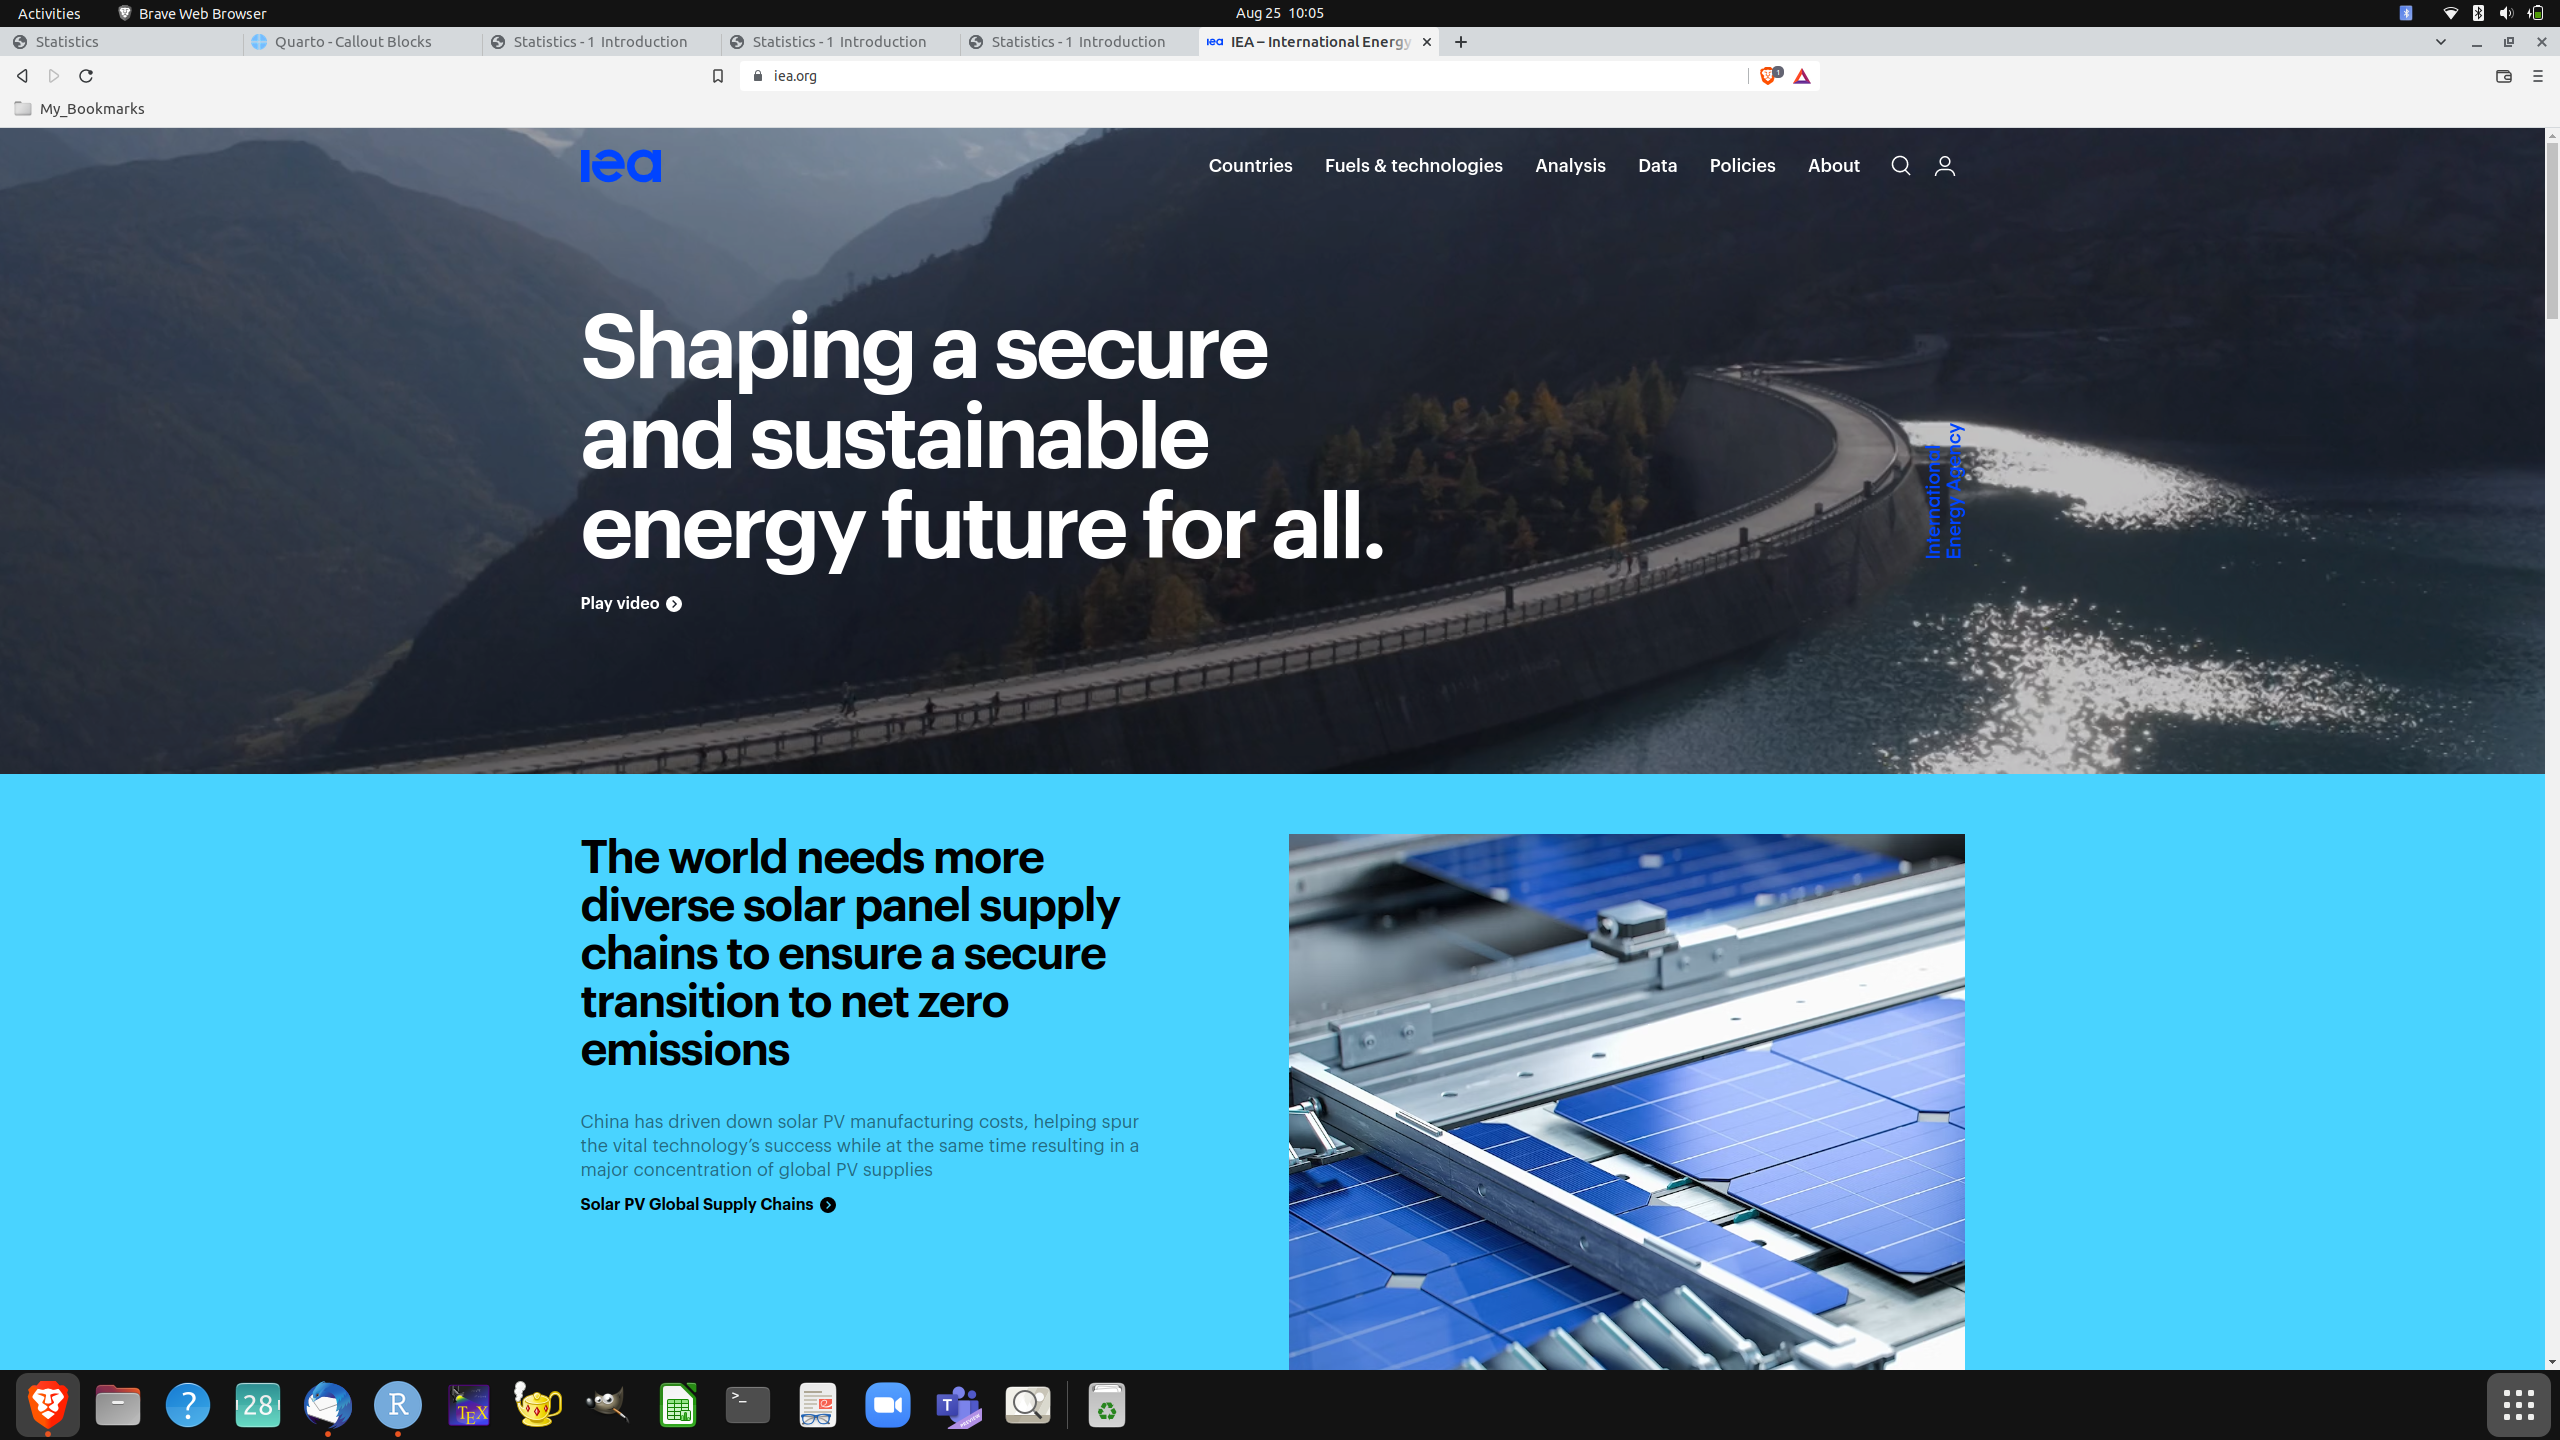
\includegraphics{./pictures/IEA-website-as-of-2022-08.png}}
\end{tcolorbox}

Now let's take a quiz and guess. What do you think is actually the
biggest source of electricity production in Kenya?

\begin{enumerate}
\def\labelenumi{\arabic{enumi}.}
\tightlist
\item
  Coal
\item
  Renewable energy
\item
  Natural gas
\end{enumerate}

\begin{tcolorbox}[enhanced jigsaw, toprule=.15mm, colbacktitle=quarto-callout-caution-color!10!white, breakable, coltitle=black, rightrule=.15mm, bottomtitle=1mm, bottomrule=.15mm, titlerule=0mm, title=\textcolor{quarto-callout-caution-color}{\faFire}\hspace{0.5em}{Seitwerk: Expand for reading comment.}, arc=.35mm, leftrule=.75mm, toptitle=1mm, left=2mm, opacityback=0, opacitybacktitle=0.6, colframe=quarto-callout-caution-color-frame, colback=white]
It would be great to make this like an online quiz, where you can click
the answer and get right or wrong. Renewable energy is the right answer.
\end{tcolorbox}

Consulting the IEA data, you will find that the correct answer is
\emph{renewable energy}. A very interesting website called
\emph{gapminder}, which analyzes the answers of many people to this
question, finds that 61 \% give a wrong answer to this question. Maybe
they find it hard to imagine that 80 \% of energy production in Kenya is
already fossil free thanks to huge sources of geothermal- and
hydropower.\sidenote{\footnotesize Geothermal electricity generation uses the earth's
  natural heating energy - geothermal energy. A country needs to be
  located on a geothermal hot spot to make effective use of this energy
  source for electricity generation. At such a hotspot there are high
  temperatures beneath the earth's surface which naturally produces
  steam. This steam can be used to spin turbines connected to a
  generator. This mechanism then produces electricity. Hydropower uses
  the water cycle to generate electricity by using dams to alter the
  flow of a river. The kinetic energy of the water spins turbines
  connected to a generator which produces electricity.} Even if you
break the answers down by country you see that 38 \% of people from
Kenya get the answer wrong. Among the people from the UK, who answer
this question even 72 \% answer wrongly.

If you are not familiar with the details of electricity production using
geothermal- and hydropower or if you are not completely sure how to
interpret a number like 38 \%, don't worry for now. The point here is
that you see that one useful consequence of being able to access, read
and interpret data is that it can help to establish facts about the
world. In this way data can help us to perhaps correct misconceptions we
might have had about these facts.

\begin{tcolorbox}[enhanced jigsaw, toprule=.15mm, colbacktitle=quarto-callout-tip-color!10!white, breakable, coltitle=black, rightrule=.15mm, bottomtitle=1mm, bottomrule=.15mm, titlerule=0mm, title=\textcolor{quarto-callout-tip-color}{\faLightbulb}\hspace{0.5em}{The gapminder webpage}, arc=.35mm, leftrule=.75mm, toptitle=1mm, left=2mm, opacityback=0, opacitybacktitle=0.6, colframe=quarto-callout-tip-color-frame, colback=white]
If you have internet access you can reach the gapminder webpage at
https://www.gapminder.org/. I encourage you to visit this page at an
occasion when you have access to the internet. You will be surprised how
often you might have a wrong guess about basic facts in the
world.\sidenote{\footnotesize Here is how the website looks like as of August 2022:
  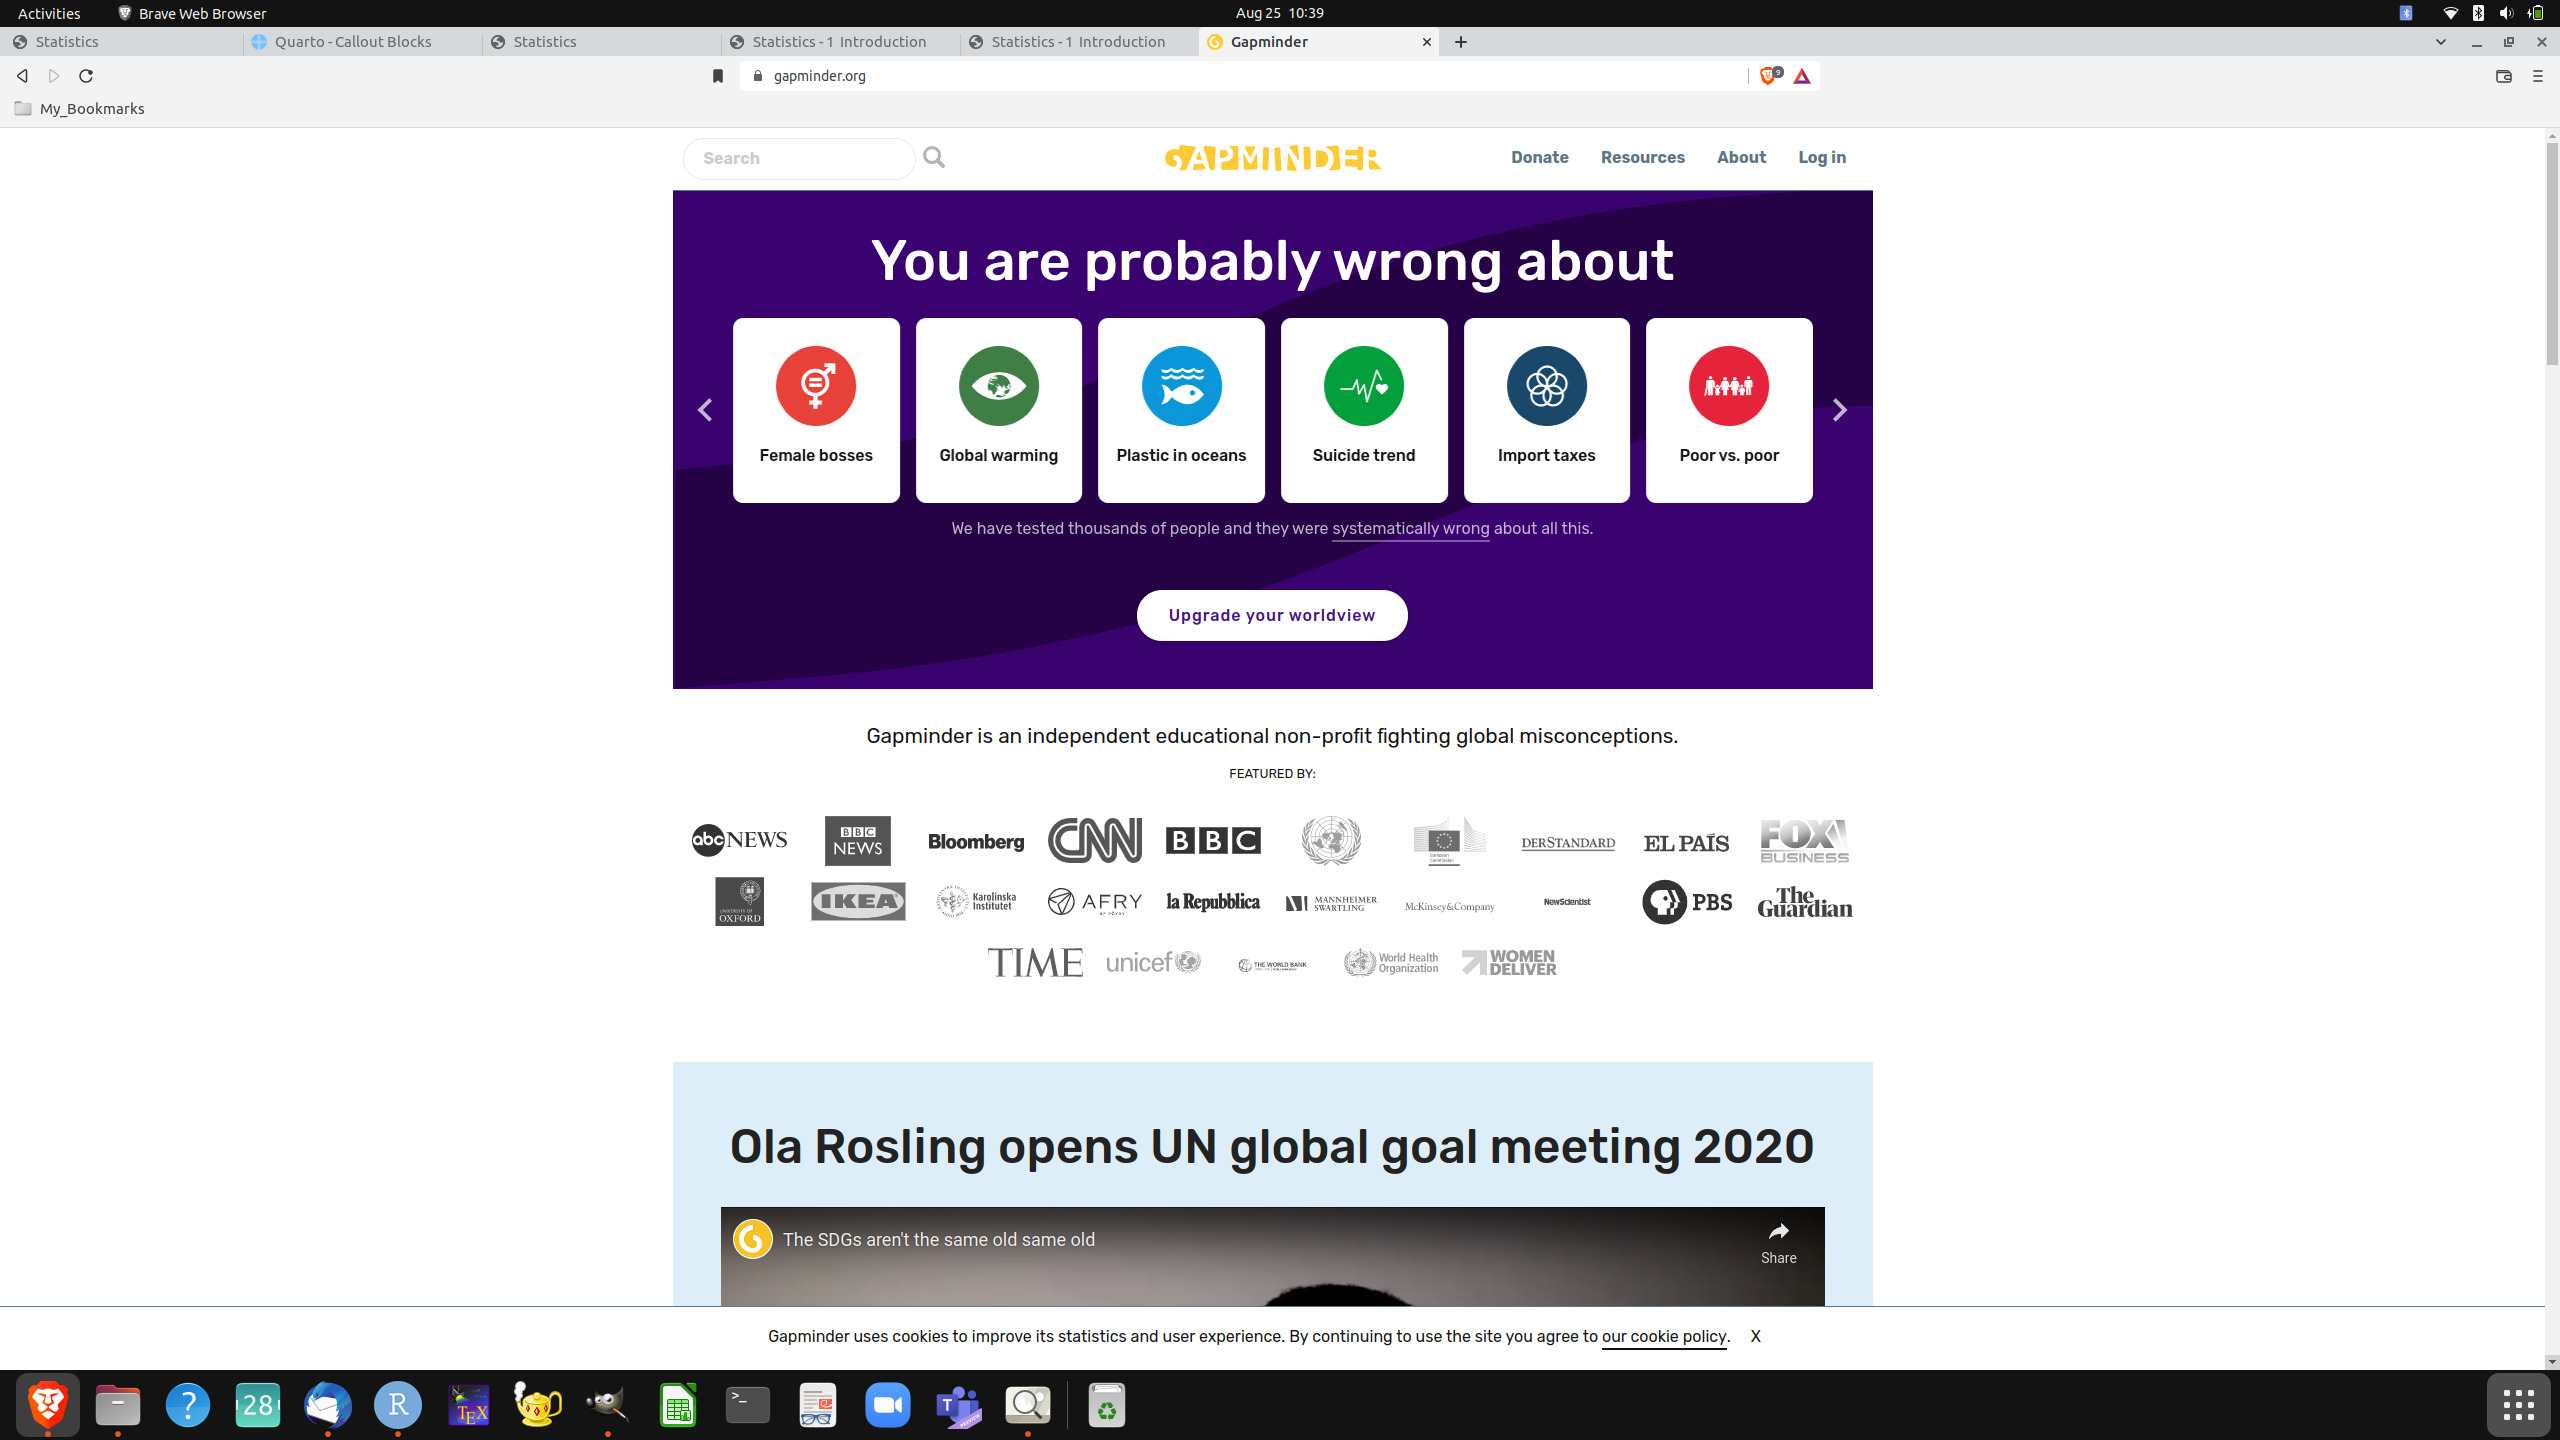
\includegraphics{./pictures/gapminder-website-as-of-2022-08.png}}
\end{tcolorbox}

In this course you will learn how to work with data and how to learn
from these data in a systematic way.

\hypertarget{how-many-trees-are-there-on-the-planet}{%
\subsection{How many trees are there on the
planet?}\label{how-many-trees-are-there-on-the-planet}}

Learning from data entails more than just establishing facts. This might
not always be possible, either because you cannot access the relevant
data or you cannot completely access them, since doing so would be way
too expensive. When working with data you also need rigorous definitions
of concepts, so that you can actually transform your experience about
the world into data

Think for a moment about the following interesting example, which I
learned from a wonderful book by the British statistician David
Spiegelhalter (Spiegelhalter 2019). The example shows that even just
categorizing and labeling things in the world to measure them and turn
them into data can be challenging. A very basic question raised in the
introduction of this book is:

\begin{tcolorbox}[enhanced jigsaw, toprule=.15mm, colbacktitle=quarto-callout-note-color!10!white, breakable, coltitle=black, rightrule=.15mm, bottomtitle=1mm, bottomrule=.15mm, titlerule=0mm, title={Question:}, arc=.35mm, leftrule=.75mm, toptitle=1mm, left=2mm, opacityback=0, opacitybacktitle=0.6, colframe=quarto-callout-note-color-frame, colback=white]
How many trees are there on the planet?
\end{tcolorbox}

It is clear that answering this question is more challenging than the
task the IEA had to solve when listing energy sources by country around
the world in a given time period. But before you go about to think how
you might count all the trees on the planet, you have to answer an even
more basic question, namely: What is a tree?

Some of you might think this is a silly and obvious question, which
every child can answer. But what some might consider a tree others will
consider just a shrub. Turning experience into data requires rigorous
definitions. It turns out that such definitions can be given for trees.
\sidenote{\footnotesize For example the forestry expert Michael Kuhns writes:
  ``\ldots{}\emph{Though no scientific definition exists to separate
  trees and shrubs, a useful definition for a tree is a woody plant
  having one erect perennial stem (trunk) at least three inches in
  diameter at a point 4-1/2 feet above the ground, a definitely formed
  crown of foliage, and a mature height of at least 13 feet. This
  definition works fine, though some trees may have more than one stem
  and young trees obviously don't meet the size criteria. A shrub can
  then be defined as a woody plant with several perennial stems that may
  be erect or may lay close to the ground. It will usually have a height
  less than 13 feet and stems no more than about three inches in
  diameter.}'' (Kuhns, n.d.)}

But even with the definition at hand you cannot just go around the
planet and count every plant that meets the criteria. So this is what
the researchers investigating that question did according to
(Spiegelhalter 2019):

``\ldots{}\emph{They first took a series of of areas with a common type
of landscape, known as a biome and counted the average number of trees
per square kilometer. They then used satellite imaging to estimate the
total area of the planet covered by each type of biome, carried out some
complex statistical modelling, and eventually came up with an estimate
of 3.04 trillion (3,040,000,000,000) trees on the planet. This sounds a
lot, except that they reckoned there used to be twice this number}.''

Now imagine that if long expert discussions are needed to precisely
define something so seemingly obvious as a tree, clearly more complex
concepts such as unemployment or the definition of the total value of
goods and services produced in a country in a given year, known as Gross
Domestic Product or GDP, is even more challenging.

There is no automatism or mechanical receipt how we can turn experience
into data and the statistics that we use and produce are constructed on
the basis of judgement. It is a starting point for a deeper
understanding of the world around us. This is one of the reasons why in
this course statistics is not only referred to as science, which it
arguably is to some degree, but also as an art.

To guard against the trap of mindlessly fall into mechanical thinking or
automatism it is sometimes helpful to make a rough plausibility
estimates about the order of magnitude you might expect as a result for
a really big number, like the number of trees on the globe.

\begin{tcolorbox}[enhanced jigsaw, toprule=.15mm, colbacktitle=quarto-callout-caution-color!10!white, breakable, coltitle=black, rightrule=.15mm, bottomtitle=1mm, bottomrule=.15mm, titlerule=0mm, title=\textcolor{quarto-callout-caution-color}{\faFire}\hspace{0.5em}{Comment for Seitwerk: Please uncollapse}, arc=.35mm, leftrule=.75mm, toptitle=1mm, left=2mm, opacityback=0, opacitybacktitle=0.6, colframe=quarto-callout-caution-color-frame, colback=white]
Here would be a good opportunity to engage students in an activity
estimating a big number. Since this has an interactive part, which
better works when in class together, one could set up the problem with
some guidance in the online unit and then discuss solutions in class. It
might be fun to add a competitive element by splitting the students in
teams or pairs and rewarding the team/pair who comes closest to the true
value. Let them first just guess and then lead them through the
guestimation a bit more systematically: One way to lead students through
this exercise might be: How many people are there in country X, how many
children of school age, how many of them ride the bus, how many students
can be transported by a bus etc. The estimate will have lots of
uncertainty but be hopefully closer to the truth than most of the
original unguided guesses. It is a first encounter for the students with
propagation of uncertainty, an important topic in statistics more
generally. The activity contains further interesting aspects like
reliability of data sources and the design of data collection. I am not
quite sure whether and how to build this in at this stage but maybe you
have an idea or suggestion.

A good example would for instance be: How many school buses are there in
country X?
\end{tcolorbox}

\hypertarget{what-has-happened-to-extreme-poverty-on-the-globe-in-the-last-20-years}{%
\subsection{What has happened to extreme poverty on the globe in the
last 20
years?}\label{what-has-happened-to-extreme-poverty-on-the-globe-in-the-last-20-years}}

One of the limitations of data as a source of knowledge about the world
is that anything we choose to measure will differ across places, across
persons or across time. When analyzing and trying to understand data we
will always face the problem how we can extract meaningful insights from
this apparent random variation. One challenge faced by statistics and
one core topic in this course will thus be how we can distinguish in
data the important relationships from the unimportant background
variability.

Exploring and finding such meaningful relationships or patterns in data
using the science of statistics and computational tools is one of the
skills you will learn in this course.

An example of a pattern in data is if we can spot a trend, data values
which are for example increasing or decreasing.

Consider the following data from the World Bank, reporting the share of
people in the world who are living in extreme poverty. Extreme poverty
is defined by the World Bank, an international development finance
organisation for low and middle income countries located in the
US\sidenote{\footnotesize The Worldbank is an international financial institution
  founded along with the International Monetary Fund in the Bretton Wods
  conference in 1944. It is located in Washington D.C. and finances
  projects in low and middle income countries. It also collects and
  processes data globally to support its activities and conduct
  development research. The Worldbank makes its data public in print or
  through its website https://www.worldbank.org/en/home} as the
percentage of people in the world who have to live on less that \$ 1.90
per day.

Let us have a look at a table showing the first 10 observations of this
share

\begin{Shaded}
\begin{Highlighting}[]
\CommentTok{\# read poverty data from our project data folder}
\NormalTok{povdat\_by\_country }\OtherTok{\textless{}{-}} \FunctionTok{read.csv}\NormalTok{(}\StringTok{"data/extreme\_poverty/share{-}of{-}population{-}in{-}extreme{-}poverty.csv"}\NormalTok{)}
\CommentTok{\# select the years from 2000}
\NormalTok{povdat\_world }\OtherTok{\textless{}{-}} \FunctionTok{with}\NormalTok{(povdat\_by\_country, povdat\_by\_country[Entity }\SpecialCharTok{==} \StringTok{"World"} \SpecialCharTok{\&}\NormalTok{ Year }\SpecialCharTok{\textgreater{}=} \DecValTok{2000}\NormalTok{, ])}
\CommentTok{\# Keep only the year and the share}
\NormalTok{plot\_data }\OtherTok{\textless{}{-}}\NormalTok{ povdat\_world[,}\FunctionTok{c}\NormalTok{(}\DecValTok{3}\NormalTok{,}\DecValTok{4}\NormalTok{)]}
\CommentTok{\# Rename variables}
\FunctionTok{names}\NormalTok{(plot\_data) }\OtherTok{\textless{}{-}} \FunctionTok{c}\NormalTok{(}\StringTok{"Year"}\NormalTok{, }\StringTok{"Share"}\NormalTok{)}

\CommentTok{\# produce a table}
\FunctionTok{library}\NormalTok{(knitr)}
\FunctionTok{kable}\NormalTok{(}\FunctionTok{head}\NormalTok{(plot\_data, }\AttributeTok{n=} \DecValTok{10}\NormalTok{), }\AttributeTok{row.names =}\NormalTok{ F, }\AttributeTok{digits =} \DecValTok{1}\NormalTok{)}
\end{Highlighting}
\end{Shaded}

\hypertarget{tbl-example-poverty}{}
\begin{longtable}[]{@{}rr@{}}
\caption{\label{tbl-example-poverty}Share of world polpulation living in
extreme poverty, Source: World Bank}\tabularnewline
\toprule()
Year & Share \\
\midrule()
\endfirsthead
\toprule()
Year & Share \\
\midrule()
\endhead
2000 & 27.8 \\
2001 & 26.9 \\
2002 & 25.7 \\
2003 & 24.7 \\
2004 & 22.9 \\
2005 & 21.0 \\
2006 & 20.3 \\
2007 & 19.1 \\
2008 & 18.4 \\
2009 & 17.6 \\
\bottomrule()
\end{longtable}

\begin{Shaded}
\begin{Highlighting}[]
\FunctionTok{write.csv}\NormalTok{(}\FunctionTok{head}\NormalTok{(plot\_data, }\AttributeTok{n=} \DecValTok{10}\NormalTok{), }\AttributeTok{file =} \StringTok{"tables/table\_1\_1\_world\_poverty.csv"}\NormalTok{, }\AttributeTok{row.names =} \ConstantTok{FALSE}\NormalTok{)}
\end{Highlighting}
\end{Shaded}

The table shows that the share of people living in extreme poverty has
been decreasing year after year for the first 10 years since the year
2000. This is a pattern which is called a \emph{downward trend}.

Note that we did not show the whole series of numbers. The data points
in our data-set actually range until the year 2017. Printing them all in
a table quickly produces very large and unwieldy number array which is
awkward to read.

Exploring data and detecting patterns is usually easier when we use the
power of the human visual system. Humans are very good in finding visual
patterns. Looking for patterns is almost visceral for us. We can't help
but looking for patterns. This almost instinctive human urge can also be
misleading and suggesting patterns to us where there are in fact none.

In data exploration we can make use of the power of visualization by
plotting data and looking at them graphically. The modern computer has
made this form of displaying data particularly easy and powerful and
visualizing data in data exploration is another core skill you are going
to learn in this course.

So let us visualize the world poverty data. In our plot we draw the year
on the x-axes and the share of people living in extreme poverty on the
y-axes. This will give us a point for each year. To facilitate the
spotting of a trend, we connect the annual observations by a line.

\begin{Shaded}
\begin{Highlighting}[]
\FunctionTok{library}\NormalTok{(ggplot2)}

\NormalTok{p }\OtherTok{\textless{}{-}} \FunctionTok{ggplot}\NormalTok{(plot\_data, }\FunctionTok{aes}\NormalTok{(}\AttributeTok{x =}\NormalTok{ Year, }\AttributeTok{y =}\NormalTok{ Share)) }\SpecialCharTok{+} 
     \FunctionTok{geom\_line}\NormalTok{() }\SpecialCharTok{+}
     \FunctionTok{geom\_point}\NormalTok{() }\SpecialCharTok{+}
     \FunctionTok{xlab}\NormalTok{(}\StringTok{""}\NormalTok{)}
\FunctionTok{ggsave}\NormalTok{(}\AttributeTok{plot=}\NormalTok{p, }\AttributeTok{filename=}\StringTok{"figures/fig{-}share{-}of{-}people{-}in{-}extreme{-}poverty{-}world.png"}\NormalTok{)}
\NormalTok{p}
\end{Highlighting}
\end{Shaded}

\begin{figure}[H]

{\centering 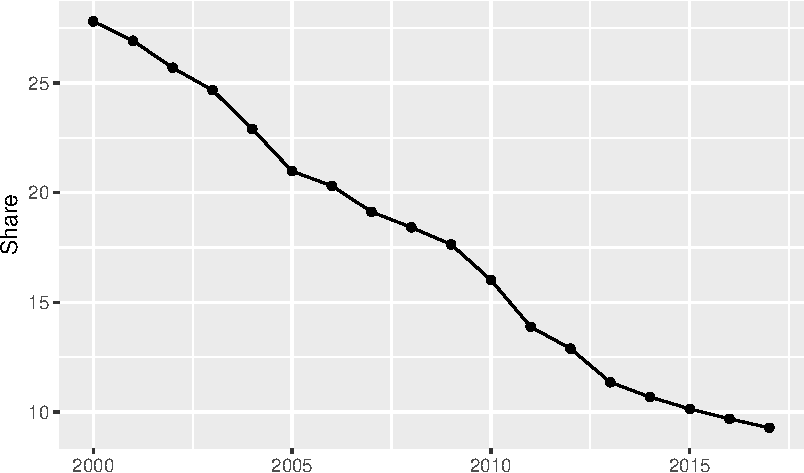
\includegraphics{./introduction_files/figure-pdf/fig-share-of-people-in-extreme-poverty-world-1.pdf}

}

\caption{\label{fig-share-of-people-in-extreme-poverty-world}Share of
world population living in extreme poverty from 2000 - 2017}

\end{figure}

Visualizing trends in world extreme poverty as an example of data
exploration. In this case the data pattern reveals a stunning fact. Over
almost two decades we can see a sharp fall in the share of extremely
poor people when looked at from a global perspective.

Of course when we drill down to the level of individual countries this
trend will not look the same everywhere and there might be countries
where the share has actually increased. But overall we have seen a
breathtaking steady decline. This is good news.\sidenote{\footnotesize When you have
  access to the internet you can have a closer look at these data at the
  very interesting website ``our world in data'' maintained by a
  consortium of Oxford University and University College London. See
  https://ourworldindata.org/extreme-poverty. The website has many
  interesting visualizations and options to select individual countries,
  country aggregates and make other selections of the data.}

But does this trend mean that extreme poverty must disappear some years
down the road? No, because nobody can tell whether the trend of the last
two decades will go on also in the future.

Statistics can help us to think more systematically about patterns and
in making systematic guesses how a pattern might continue in the future.
This is another core skill you will learn in this course: Making
predictions, which means using available data and information to make
informed guesses about data and information we do not have.

Let us go back to the share of people in the world living in extreme
poverty. As reported in our data the last actual observation for the
global share in extreme poverty from the world bank is from 2017. There
are more recent data for some regions but the global data since then are
by now forecasts based on statistical techniques. The basic ideas of
these techniques and how to apply them to data is a core skill you will
learn in this course.

Now what does the World bank predict for the share of extreme poverty in
the world? Let us look at the data again graphically to visualize the
prediction.

\begin{Shaded}
\begin{Highlighting}[]
\NormalTok{obsdat }\OtherTok{\textless{}{-}} \FunctionTok{data.frame}\NormalTok{(}\AttributeTok{Year =}\NormalTok{ plot\_data}\SpecialCharTok{$}\NormalTok{Year, }\AttributeTok{Scenario =} \FunctionTok{rep}\NormalTok{(}\StringTok{"Observed"}\NormalTok{, }\DecValTok{18}\NormalTok{), }\AttributeTok{Share =}\NormalTok{ plot\_data}\SpecialCharTok{$}\NormalTok{Share)}

\NormalTok{add\_dat }\OtherTok{\textless{}{-}} \FunctionTok{data.frame}\NormalTok{(}\AttributeTok{Year =} \DecValTok{2018}\NormalTok{, }\AttributeTok{Scenario =} \StringTok{"Observed"}\NormalTok{, }\AttributeTok{Share =} \FloatTok{8.6}\NormalTok{)}

\NormalTok{pred\_dat\_precovid }\OtherTok{\textless{}{-}} \FunctionTok{data.frame}\NormalTok{(}\AttributeTok{Year =} \FunctionTok{c}\NormalTok{(}\DecValTok{2018}\NormalTok{, }\DecValTok{2019}\NormalTok{, }\DecValTok{2020}\NormalTok{, }\DecValTok{2021}\NormalTok{), }\AttributeTok{Scenario =} \FunctionTok{rep}\NormalTok{(}\StringTok{"Pre{-}Covid{-}19"}\NormalTok{, }\DecValTok{4}\NormalTok{), }\AttributeTok{Share =} \FunctionTok{c}\NormalTok{(}\FloatTok{8.6}\NormalTok{, }\FloatTok{8.4}\NormalTok{, }\FloatTok{7.9}\NormalTok{, }\FloatTok{7.5}\NormalTok{))}

\NormalTok{pred\_dat\_covidbase }\OtherTok{\textless{}{-}} \FunctionTok{data.frame}\NormalTok{(}\AttributeTok{Year =} \FunctionTok{c}\NormalTok{(}\DecValTok{2018}\NormalTok{, }\DecValTok{2019}\NormalTok{, }\DecValTok{2020}\NormalTok{, }\DecValTok{2021}\NormalTok{), }\AttributeTok{Scenario =} \FunctionTok{rep}\NormalTok{(}\StringTok{"Covid{-}19{-}Baseline"}\NormalTok{, }\DecValTok{4}\NormalTok{), }\AttributeTok{Share =} \FunctionTok{c}\NormalTok{(}\FloatTok{8.6}\NormalTok{, }\FloatTok{8.4}\NormalTok{, }\FloatTok{9.1}\NormalTok{, }\FloatTok{8.9}\NormalTok{))}

\NormalTok{pred\_dat\_coviddown }\OtherTok{\textless{}{-}} \FunctionTok{data.frame}\NormalTok{(}\AttributeTok{Year =} \FunctionTok{c}\NormalTok{(}\DecValTok{2018}\NormalTok{, }\DecValTok{2019}\NormalTok{, }\DecValTok{2020}\NormalTok{, }\DecValTok{2021}\NormalTok{), }\AttributeTok{Scenario =} \FunctionTok{rep}\NormalTok{(}\StringTok{"Covid{-}19{-}Downside"}\NormalTok{, }\DecValTok{4}\NormalTok{), }\AttributeTok{Share =} \FunctionTok{c}\NormalTok{(}\FloatTok{8.6}\NormalTok{, }\FloatTok{8.4}\NormalTok{, }\FloatTok{9.4}\NormalTok{, }\FloatTok{9.4}\NormalTok{))}

\NormalTok{dat }\OtherTok{\textless{}{-}} \FunctionTok{rbind}\NormalTok{(obsdat, add\_dat, pred\_dat\_precovid, pred\_dat\_covidbase, pred\_dat\_coviddown)}

\NormalTok{p }\OtherTok{\textless{}{-}} \FunctionTok{ggplot}\NormalTok{(dat, }\FunctionTok{aes}\NormalTok{(}\AttributeTok{x =}\NormalTok{ Year, }\AttributeTok{y =}\NormalTok{ Share, }\AttributeTok{group =}\NormalTok{ Scenario, }\AttributeTok{color =}\NormalTok{ Scenario)) }\SpecialCharTok{+} 
  \FunctionTok{geom\_line}\NormalTok{(}\AttributeTok{alpha =} \FloatTok{0.5}\NormalTok{)}\SpecialCharTok{+}
  \FunctionTok{geom\_point}\NormalTok{()}\SpecialCharTok{+}
  \FunctionTok{scale\_color\_manual}\NormalTok{(}\AttributeTok{values=}\FunctionTok{c}\NormalTok{(}\StringTok{\textquotesingle{}green\textquotesingle{}}\NormalTok{, }\StringTok{\textquotesingle{}red\textquotesingle{}}\NormalTok{, }\StringTok{\textquotesingle{}black\textquotesingle{}}\NormalTok{, }\StringTok{\textquotesingle{}blue\textquotesingle{}}\NormalTok{))}
\FunctionTok{ggsave}\NormalTok{(}\AttributeTok{plot=}\NormalTok{p, }\AttributeTok{filename=}\StringTok{"figures/fig{-}share{-}of{-}people{-}in{-}extreme{-}poverty{-}world{-}forecast.png"}\NormalTok{)}
\NormalTok{p}
\end{Highlighting}
\end{Shaded}

\begin{figure}[H]

{\centering 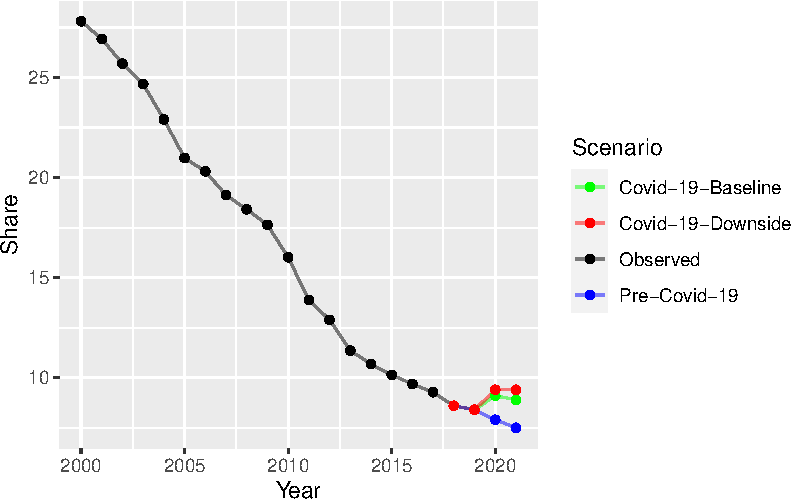
\includegraphics{./introduction_files/figure-pdf/fig-share-of-people-in-extreme-poverty-world-forecast-1.pdf}

}

\caption{\label{fig-share-of-people-in-extreme-poverty-world-forecast}Share
of world population living in extreme poverty from 2000 - 2017 with
predictions until 2021}

\end{figure}

Observe that the line showing the share of extreme poverty in the world
takes different distinct future paths as we make predictions. What does
this mean?

At the root of the predictions is an abstract model\sidenote{\footnotesize If you have
  difficulties now to imagine what this means, don't worry. We will
  learn in detail what a model is and how it can be interpret. In
  practice a model is usually an equation which provides a
  low-dimensional summary of a dataset. This summary is then used to
  make predictions.}, how the share of poverty changes over time. If the
underlying data would correspond to a world before Covid the falling
trend in poverty would just continue to fall, as it has done
continuously from 2000 onward. In the graph you can see this scenario if
you follow the black and the blue line. But taking the pandemic and the
consequences into account the prediction of the World Bank is that
extreme poverty after a almost two decades downward trend will rise
again. This you can see by following the green and the red line. How
much, this rise actually will be in the end depends on data we can not
yet know.

When we make informed guesses based on observed data on information we
do not yet have there is uncertainty involved. Using the theory of
probability in combination with statistics we can quantify this
uncertainty. Quantifying the uncertainty attached to predictions is the
third basic skill you will learn in this course.

\hypertarget{does-taking-your-time-in-college-pay-off}{%
\subsection{Does taking your time in college pay
off?}\label{does-taking-your-time-in-college-pay-off}}

A newspaper in Germany reported that the more semesters needed to
complete an academic program at the university the greater the starting
salary in the first year of a job. The report was based on a study that
used a random sample\sidenote{\footnotesize We will later in the course learn in
  detail what a random sample is. For the moment imagine that there is a
  mechanism which allows to select these 24 students at random from the
  large population of all university students in Germany. When a sample
  is random, every member in the sample has the same probability of
  beeing chosen from the population.} of 24 people who had recently
completed an academic program.

Information was collected on the number of semesters each person in the
sample needed to complete the program and the starting salary, in
thousand Euros, at the beginning of the job.

The data are shown in the following plot

\begin{Shaded}
\begin{Highlighting}[]
\NormalTok{dat }\OtherTok{\textless{}{-}} \FunctionTok{read.csv}\NormalTok{(}\StringTok{"data/college\_years\_salaries/coll\_sal.csv"}\NormalTok{)}

\FunctionTok{library}\NormalTok{(ggplot2)}

\NormalTok{p }\OtherTok{\textless{}{-}} \FunctionTok{ggplot}\NormalTok{(dat, }\FunctionTok{aes}\NormalTok{(}\AttributeTok{x=}\NormalTok{Time, }\AttributeTok{y=}\NormalTok{Salary)) }\SpecialCharTok{+}
     \FunctionTok{geom\_point}\NormalTok{()}
\FunctionTok{ggsave}\NormalTok{(}\AttributeTok{plot=}\NormalTok{p, }\AttributeTok{filename=}\StringTok{"figures/Years\_in\_college\_versus\_starting\_salary.png"}\NormalTok{)}
\NormalTok{p}
\end{Highlighting}
\end{Shaded}

\begin{figure}[H]

{\centering 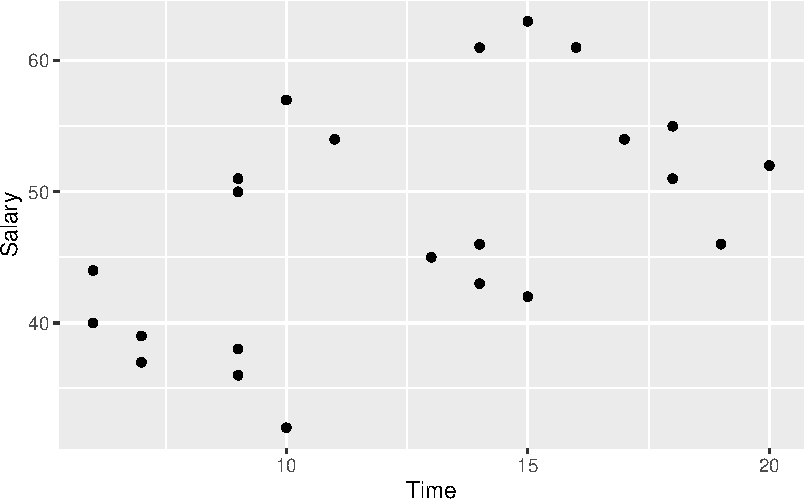
\includegraphics{./introduction_files/figure-pdf/Years_in_college_versus_starting_salary-1.pdf}

}

\caption{Relation between the semesters needed by a random sample of 24
German students to complete an academic university programm and the
starting salary in the first year in the job.}

\end{figure}

What you see in this picture is a so called \emph{scatter-plot}. It
takes the data and plots all pairs of time in semesters needed to
complete the academic university program and the starting salary in the
job, where the first value is shown on the x-axis and the second on the
y-axes. The points you draw like this are ``scattered'' all over the
place, but it seems that ``by and large'' there is also some trend -
shown as a blue line - like this:

\begin{Shaded}
\begin{Highlighting}[]
\NormalTok{p }\OtherTok{\textless{}{-}} \FunctionTok{ggplot}\NormalTok{(dat, }\FunctionTok{aes}\NormalTok{(}\AttributeTok{x=}\NormalTok{Time, }\AttributeTok{y=}\NormalTok{Salary)) }\SpecialCharTok{+}
     \FunctionTok{geom\_point}\NormalTok{() }\SpecialCharTok{+}
     \FunctionTok{geom\_smooth}\NormalTok{(}\AttributeTok{method =} \StringTok{"lm"}\NormalTok{, }\AttributeTok{se =} \ConstantTok{FALSE}\NormalTok{)}
\FunctionTok{ggsave}\NormalTok{(}\AttributeTok{plot=}\NormalTok{p, }\AttributeTok{filename=}\StringTok{"figures/Years\_in\_college\_versus\_starting\_salary\_with\_trend.png"}\NormalTok{)}
\NormalTok{p}
\end{Highlighting}
\end{Shaded}

\begin{figure}[H]

{\centering 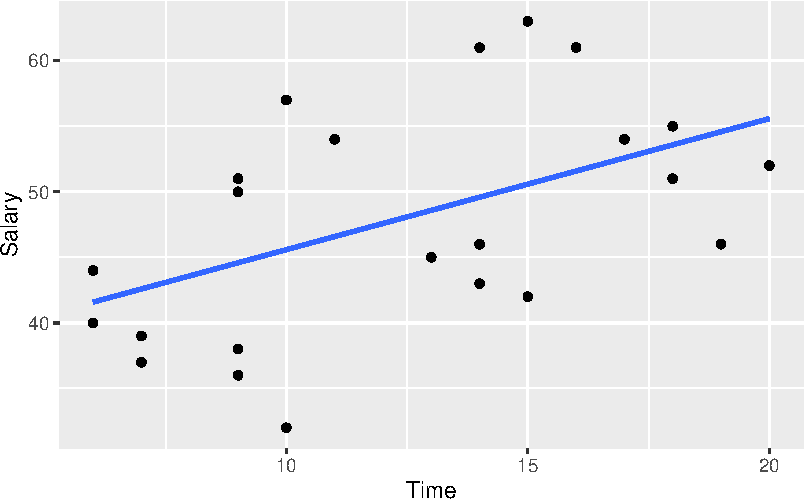
\includegraphics{./introduction_files/figure-pdf/Years in college versus starting salary with trend-1.pdf}

}

\caption{Relation between the semesters needed by a random sample of 24
German students to complete an academic university programm and the
starting salary in the first year in the job with a linear trend fitted
to data.}

\end{figure}

Looking at the data, does this plot support the claim of the Newspaper?

Apparently the journalist writing the article saw a pattern, shown here
as the blue line, which suggests that on average the salaries are really
increasing with the semesters spent at the university. But is this
pattern plausible? What do you think?

An independent researcher, who doubted the result, received the data
from the newspaper and did a new analysis by separating the data into
three groups based on the major of each person.

\begin{Shaded}
\begin{Highlighting}[]
\NormalTok{p }\OtherTok{\textless{}{-}} \FunctionTok{ggplot}\NormalTok{(dat, }\FunctionTok{aes}\NormalTok{(}\AttributeTok{x=}\NormalTok{Time, }\AttributeTok{y=}\NormalTok{Salary, }\AttributeTok{group =}\NormalTok{ Major, }\AttributeTok{color =}\NormalTok{ Major)) }\SpecialCharTok{+}
     \FunctionTok{geom\_point}\NormalTok{()}
\FunctionTok{ggsave}\NormalTok{(}\AttributeTok{plot=}\NormalTok{p, }\AttributeTok{filename=}\StringTok{"figures/Years\_in\_college\_versus\_starting\_salary\_by\_major.png"}\NormalTok{)}
\NormalTok{p}
\end{Highlighting}
\end{Shaded}

\begin{figure}[H]

{\centering 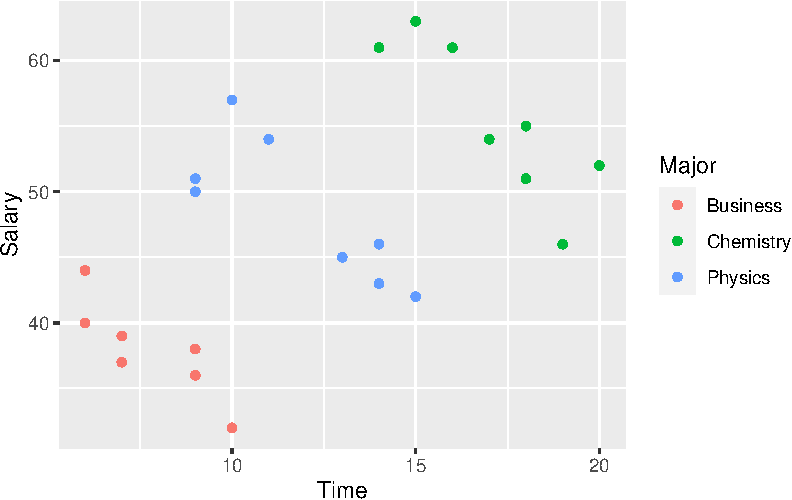
\includegraphics{./introduction_files/figure-pdf/Years_in_college_versus_starting_salary_by_major-1.pdf}

}

\caption{Relation between the semesters needed by a random sample of 24
German students to complete an academic university programm by major and
the starting salary in the first year in the job.}

\end{figure}

Now, looking at this plot, describe the relation for students with a
major in business. How could the newspaper report be modified to
describe the data?

\begin{tcolorbox}[enhanced jigsaw, toprule=.15mm, colbacktitle=quarto-callout-caution-color!10!white, breakable, coltitle=black, rightrule=.15mm, bottomtitle=1mm, bottomrule=.15mm, titlerule=0mm, title=\textcolor{quarto-callout-caution-color}{\faFire}\hspace{0.5em}{Comment for Seitwerk}, arc=.35mm, leftrule=.75mm, toptitle=1mm, left=2mm, opacityback=0, opacitybacktitle=0.6, colframe=quarto-callout-caution-color-frame, colback=white]
This example works particularly well for involving students. I am not
quiet sure how to build this interactive element in the online unit.
maybe you have an idea.
\end{tcolorbox}

You see in this example that looking for patterns is not as easy as it
seems. Again we see that there are no automatism. You will need the
skills you learn in this course to gain competence in distinguishing
actual patterns from spurious ones.

Why did I go through all these example with you in the beginning,
pinning down the share of renewable energy in the electricity production
in Kenya, estimating the number of trees on the planet, long term trends
in world extreme poverty, and the relation between study time and
beginning salaries for students in Germany? All these examples
illustrate some special skills you will learn in this course. Hopefully
it also convinced most of you that statistics and working with data is
an exciting field and a way to engage with real world issues.

So these are the three core skills you will learn in this course:

\hypertarget{the-three-basic-skills-you-will-learn-in-this-course}{%
\section{The three basic skills you will learn in this
course}\label{the-three-basic-skills-you-will-learn-in-this-course}}

\begin{tcolorbox}[enhanced jigsaw, toprule=.15mm, colbacktitle=quarto-callout-important-color!10!white, breakable, coltitle=black, rightrule=.15mm, bottomtitle=1mm, bottomrule=.15mm, titlerule=0mm, title=\textcolor{quarto-callout-important-color}{\faExclamation}\hspace{0.5em}{The three basic skills you will learn in this course}, arc=.35mm, leftrule=.75mm, toptitle=1mm, left=2mm, opacityback=0, opacitybacktitle=0.6, colframe=quarto-callout-important-color-frame, colback=white]

After successfully completing this course students you will have learned
three core skills:

\begin{enumerate}
\def\labelenumi{\arabic{enumi}.}
\item
  \textbf{Data exploration} or finding patterns in data and information
  through visualisation and computation.
\item
  \textbf{Making predictions}, which means using available data and
  information to make informed guesses about data and information we do
  not have.
\item
  To \textbf{quantify the uncertainty} we have to attach to our
  predictions.
\end{enumerate}

\end{tcolorbox}

The course is split into 8 units in total. Units 1, 2 and 3 will be
mostly be concerned with data exploration and with making comparisons
based on data. You will also learn step by step how you can use the
computer for data exploration and visualization. We assume no prior
knowledge and start from scratch. We also do not strive for
completeness. The idea is that you acquire the practically most
important skills and get maturity to drill deeper for yourself after the
course either in your further studies or on the job.

Unit 4 and unit 5 will be predominantly be concerned with models and
using models for prediction. Here you will learn how to spot trends in
data, how you can discern actual information in data, so called signals,
from random variation, called noise.

Units 6, 7 and 8 will focus on how to quantify uncertainty related to
prediction and inference from data. Here is the place where probability
theory combines with statistics to provide analytically and practically
powerful tools which ground data analysis in a firm scientific
foundation. This is also the most challenging part of the course and it
will require lots of practice and participation from you to acquire this
important skill.

\begin{tcolorbox}[enhanced jigsaw, toprule=.15mm, colbacktitle=quarto-callout-caution-color!10!white, breakable, coltitle=black, rightrule=.15mm, bottomtitle=1mm, bottomrule=.15mm, titlerule=0mm, title=\textcolor{quarto-callout-caution-color}{\faFire}\hspace{0.5em}{Comment for Seitwerk}, arc=.35mm, leftrule=.75mm, toptitle=1mm, left=2mm, opacityback=0, opacitybacktitle=0.6, colframe=quarto-callout-caution-color-frame, colback=white]

In your template you suggest that in the introduction I give a minute
overview of the details of topics learned in the course. I would prefer
to abstain from this, because it contains lot of terms the students will
learn step by step and it is probably boring at this stage. I would
rather prefer the big picture approach outlined here with the three
basic skills as the guiding posts. If listing the details is a must, it
would look roughly like this:

\begin{tcolorbox}[enhanced jigsaw, toprule=.15mm, colbacktitle=quarto-callout-note-color!10!white, breakable, coltitle=black, rightrule=.15mm, bottomtitle=1mm, bottomrule=.15mm, titlerule=0mm, title=\textcolor{quarto-callout-note-color}{\faInfo}\hspace{0.5em}{Unit 1: Overview; Categorical Data and Proportions}, arc=.35mm, leftrule=.75mm, toptitle=1mm, left=2mm, opacityback=0, opacitybacktitle=0.6, colframe=quarto-callout-note-color-frame, colback=white]
In unit 1 we will give an overview of the course and we begin with the
analysis and understanding of binary variables, variables that can be
imagined as simple yes or no questions and how they can be summarized as
proportions or percentages. You will learn about how the idea of
expected frequency will promote the understanding of the meaning of
these shares and how this provides a basic understanding of the
importance of these numbers.
\end{tcolorbox}

\begin{tcolorbox}[enhanced jigsaw, toprule=.15mm, colbacktitle=quarto-callout-note-color!10!white, breakable, coltitle=black, rightrule=.15mm, bottomtitle=1mm, bottomrule=.15mm, titlerule=0mm, title=\textcolor{quarto-callout-note-color}{\faInfo}\hspace{0.5em}{Unit 2: Summarizing and Communication lots of data; From limited data to
populations}, arc=.35mm, leftrule=.75mm, toptitle=1mm, left=2mm, opacityback=0, opacitybacktitle=0.6, colframe=quarto-callout-note-color-frame, colback=white]
In unit 2 we learn how to deal with lots of data, the typical situation
we will face when we do statistics. When there are lots of data we need
instruments and tools to summarize them and to get an overview. This
overview is usually also very important for communicating the data and
the information they might contain. We will also learn how we can use
statistics to learn properties about large populations by only making
limited observations on some appropriately chosen subset of individuals
from this population. The gold standard in making such inferences
possible is the concept of a so called random sample. But at each step
of the sampling procedure bias can crop up and invalidate our results
leading to wrong conclusions. The circumstances under which inference
from samples to populations can be made and how we can make sure to
minimize bias we need a firm understanding of the opportunities and
limits of this important technique.
\end{tcolorbox}

\begin{tcolorbox}[enhanced jigsaw, toprule=.15mm, colbacktitle=quarto-callout-note-color!10!white, breakable, coltitle=black, rightrule=.15mm, bottomtitle=1mm, bottomrule=.15mm, titlerule=0mm, title=\textcolor{quarto-callout-note-color}{\faInfo}\hspace{0.5em}{Unit 3: What causes what?}, arc=.35mm, leftrule=.75mm, toptitle=1mm, left=2mm, opacityback=0, opacitybacktitle=0.6, colframe=quarto-callout-note-color-frame, colback=white]
In unit 3 we discuss when data analysis allows us to say something about
what causes what. We learn about the important concept of randomized
trials. We will also learn what an observational study is and how it
differs from a randomized trial. This is an important concept we will
learn through the discussion of real world examples.
\end{tcolorbox}

\begin{tcolorbox}[enhanced jigsaw, toprule=.15mm, colbacktitle=quarto-callout-note-color!10!white, breakable, coltitle=black, rightrule=.15mm, bottomtitle=1mm, bottomrule=.15mm, titlerule=0mm, title=\textcolor{quarto-callout-note-color}{\faInfo}\hspace{0.5em}{Unit 4: Modelling relationships using regression and algorithmic
predictions}, arc=.35mm, leftrule=.75mm, toptitle=1mm, left=2mm, opacityback=0, opacitybacktitle=0.6, colframe=quarto-callout-note-color-frame, colback=white]
In unit 4 we will learn a key concept needed to make predictions. The
technical term for this concept in statistics is regression. It is a
simple mathematical model describing how a set of explanatory variables
varies systematically with a response variable. We will learn to
construct such models and to interpret them correctly. We will also
cover related techniques which have become very important recently and
entered the statistical toolbox from the field of computer science.
These methods are known under the notion of algorithmic prediction or
machine learning.
\end{tcolorbox}

\begin{tcolorbox}[enhanced jigsaw, toprule=.15mm, colbacktitle=quarto-callout-note-color!10!white, breakable, coltitle=black, rightrule=.15mm, bottomtitle=1mm, bottomrule=.15mm, titlerule=0mm, title=\textcolor{quarto-callout-note-color}{\faInfo}\hspace{0.5em}{Unit 5: How sure can we be about what is going on: Estimates and
Intervals.}, arc=.35mm, leftrule=.75mm, toptitle=1mm, left=2mm, opacityback=0, opacitybacktitle=0.6, colframe=quarto-callout-note-color-frame, colback=white]
In unit 5 we encounter the first time tools for quantifying uncertainty.
We learn how to determine and use uncertainty intervals by using a
technique which is called the bootstrap. Being able to determine such
intervals is extremely important in communicating statistics and for
supporting a systematic and sound answer to the question: How sure can
we be about an estimate.
\end{tcolorbox}

\begin{tcolorbox}[enhanced jigsaw, toprule=.15mm, colbacktitle=quarto-callout-note-color!10!white, breakable, coltitle=black, rightrule=.15mm, bottomtitle=1mm, bottomrule=.15mm, titlerule=0mm, title=\textcolor{quarto-callout-note-color}{\faInfo}\hspace{0.5em}{Unit 6: Probability: Quantifying uncertainty and variability}, arc=.35mm, leftrule=.75mm, toptitle=1mm, left=2mm, opacityback=0, opacitybacktitle=0.6, colframe=quarto-callout-note-color-frame, colback=white]
In unit 6 we deepen the knowledge how to quantify uncertainty by
introducing basic ideas of probability theory. Probability theory
provides a formal language and mathematics for dealing with chance
phenomena. Probability is often counter intuitive but using the idea of
expected frequency improves intuition. Probability ideas can be very
useful in statistics even if there is no explicit use of a randomizing
mechanism. Many social phenomena show a remarkable regularity in their
overall pattern while individual events are entirely unpredictable.
\end{tcolorbox}

\begin{tcolorbox}[enhanced jigsaw, toprule=.15mm, colbacktitle=quarto-callout-note-color!10!white, breakable, coltitle=black, rightrule=.15mm, bottomtitle=1mm, bottomrule=.15mm, titlerule=0mm, title=\textcolor{quarto-callout-note-color}{\faInfo}\hspace{0.5em}{Unit 7: Putting Probability and Statistics together}, arc=.35mm, leftrule=.75mm, toptitle=1mm, left=2mm, opacityback=0, opacitybacktitle=0.6, colframe=quarto-callout-note-color-frame, colback=white]
In unit 7 we put statistics and probability theory together. This allows
us to both simplify ideas and techniques how to quantify uncertainty.
The combination of the two field makes the tools for quantifying
uncertainty at the same time more powerful. Combining statistics and
probability theory is at the heart of statistics as a science. It makes
all the ideas developed in unit 1 to 6 very versatile and powerful.
\end{tcolorbox}

\begin{tcolorbox}[enhanced jigsaw, toprule=.15mm, colbacktitle=quarto-callout-note-color!10!white, breakable, coltitle=black, rightrule=.15mm, bottomtitle=1mm, bottomrule=.15mm, titlerule=0mm, title=\textcolor{quarto-callout-note-color}{\faInfo}\hspace{0.5em}{Unit 8: Answering questions and claiming discoveries}, arc=.35mm, leftrule=.75mm, toptitle=1mm, left=2mm, opacityback=0, opacitybacktitle=0.6, colframe=quarto-callout-note-color-frame, colback=white]
In unit 8 we learn how to leverage the knowledge of this course to
answer questions and to claim discoveries. You will learn how statistics
is used in the sciences and how it supports to develop our knowledge of
the world. It pulls many ideas of the whole course together and when you
have mastered this unit you have mastered all the basic skills we want
to develop in this course, data exploration, prediction and quantifying
uncertainty.
\end{tcolorbox}

\end{tcolorbox}

\hypertarget{on-the-use-of-the-computer}{%
\section{On the use of the computer}\label{on-the-use-of-the-computer}}

Our approach to teach you basic ideas of statistics and data analysis
will be very much problem and activity oriented. The application of
specific statistical techniques will be only one component in a whole
package of activities you will need to engage in when you work with data
in real world applications. Preparing data appropriately for analysis as
well as communicating the conclusions for your analysis will be
important elements of the whole process of statistical analysis. Today
these activities involve using a computer.

In this course you will also learn how to use the computer. It will play
an important role for developing your skills. We will make no
assumptions of prior knowledge of computers and programming and will
introduce the use of the computer step by step.

Using a computer requires a language in which we can tell the computer
what to do and which the computer can understand. The language of our
choice for this course is called R. It is one of the most widely used
and most powerful languages for data analysis and statistics. We will
introduce you to the language and its use step by step as we go along
and in parallel with the statistical concepts we develop.

\hypertarget{activities-in-the-study-center}{%
\section{Activities in the study
center}\label{activities-in-the-study-center}}

\hypertarget{visualizing-the-share-of-extremely-poor-people-for-different-countries}{%
\subsection{Visualizing the share of extremely poor people for different
countries}\label{visualizing-the-share-of-extremely-poor-people-for-different-countries}}

\begin{tcolorbox}[enhanced jigsaw, toprule=.15mm, colbacktitle=quarto-callout-caution-color!10!white, breakable, coltitle=black, rightrule=.15mm, bottomtitle=1mm, bottomrule=.15mm, titlerule=0mm, title=\textcolor{quarto-callout-caution-color}{\faFire}\hspace{0.5em}{Comment for Seitwerk}, arc=.35mm, leftrule=.75mm, toptitle=1mm, left=2mm, opacityback=0, opacitybacktitle=0.6, colframe=quarto-callout-caution-color-frame, colback=white]
Here we assume that students have a running R and R-Studio or R with
Jupyter Notebook or Jupyter Lab installation on their laptops at the
study center. We would give the code in a notebook with the code chunk
shown in the source file, to play with.

While we need not pin down all the details of the computational
infrastructure yet, we need a discussion how to integrate the computer
instructions into the course and the material I have to prepare for
that. I would very much prefer a minimalist solution with R and some
kind of notebook but not more.
\end{tcolorbox}

Lets go back to figure
Figure~\ref{fig-share-of-people-in-extreme-poverty-world} for a moment.
This figure has been created by the use of the computer.

In the following box you see the computer code that has read the data
from a file and then plotted the share for the world and for a
particular country, say China. Don't worry if you do not (yet)
understand the details of the code. Think of it as a language that tells
the computer what to do with the data. You can edit the code and delete
China and insert another country instead. If you click the green arrow
at the upper right corner of the box the computer will run the code
again and generate a new graphic.

\begin{tcolorbox}[enhanced jigsaw, toprule=.15mm, colbacktitle=quarto-callout-caution-color!10!white, breakable, coltitle=black, rightrule=.15mm, bottomtitle=1mm, bottomrule=.15mm, titlerule=0mm, title=\textcolor{quarto-callout-caution-color}{\faFire}\hspace{0.5em}{Comment for Seitwerk}, arc=.35mm, leftrule=.75mm, toptitle=1mm, left=2mm, opacityback=0, opacitybacktitle=0.6, colframe=quarto-callout-caution-color-frame, colback=white]
The details of this will of course depend on the kind of notebook we
use. We can use in principle three options. Option 1: Have an
installation of Rstudio (https://www.rstudio.com/). RStudio is the most
popular (and free) IDE for development of R code. In R Studio we can
open quarto notebooks (qdm) and run code interactively there. Pro: Works
seamlessly with my notes and enhances production efficiency. Con: You
need to explain students the IDE in addition to R, though no big deal it
is an additional complication. Option 2: Jupyter Notebook with an R
kernel (ipynp). Pro: If JWE decides to work more with Jupyter notebooks
on a broader base, seamless integration for this strategy. Con: same as
with R studio and just a tiny inch more awkward to produce for me.
Option 3: Work in the R console only. Pro: No IDE or notebook. Con:
perhaps a bit too difficult to use for students without Computer Science
background.
\end{tcolorbox}

Try to play and experiment with the code in this way to see what
happens. Soon you will know yourself how to make interesting and
beautiful data visualizations yourself.

\begin{Shaded}
\begin{Highlighting}[]
\FunctionTok{library}\NormalTok{(ggplot2)}

\NormalTok{demo\_data }\OtherTok{\textless{}{-}} \FunctionTok{read.csv}\NormalTok{(}\StringTok{"data/extreme\_poverty/share{-}of{-}population{-}in{-}extreme{-}poverty.csv"}\NormalTok{)}

\FunctionTok{names}\NormalTok{(demo\_data) }\OtherTok{\textless{}{-}} \FunctionTok{c}\NormalTok{(}\StringTok{"Country"}\NormalTok{, }\StringTok{"Code"}\NormalTok{, }\StringTok{"Year"}\NormalTok{, }\StringTok{"Share"}\NormalTok{)}

\NormalTok{pl\_dat }\OtherTok{\textless{}{-}} \FunctionTok{with}\NormalTok{(demo\_data, demo\_data[Country }\SpecialCharTok{\%in\%} \FunctionTok{c}\NormalTok{(}\StringTok{"World"}\NormalTok{, }\StringTok{"China"}\NormalTok{) }\SpecialCharTok{\&}\NormalTok{ Year }\SpecialCharTok{\textgreater{}=} \DecValTok{2000}\NormalTok{, ])}

\NormalTok{p }\OtherTok{\textless{}{-}} \FunctionTok{ggplot}\NormalTok{(pl\_dat, }\FunctionTok{aes}\NormalTok{(}\AttributeTok{x =}\NormalTok{ Year, }\AttributeTok{y =}\NormalTok{ Share, }\AttributeTok{color =}\NormalTok{ Country)) }\SpecialCharTok{+}
     \FunctionTok{geom\_point}\NormalTok{() }\SpecialCharTok{+}
     \FunctionTok{geom\_line}\NormalTok{() }\SpecialCharTok{+}
     \FunctionTok{xlab}\NormalTok{(}\StringTok{""}\NormalTok{)}

\NormalTok{p}
\end{Highlighting}
\end{Shaded}

\begin{figure}[H]

{\centering 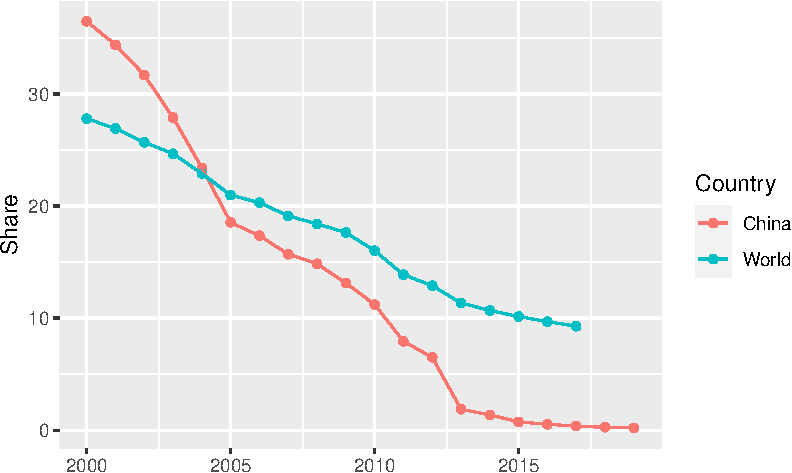
\includegraphics{./introduction_files/figure-pdf/unnamed-chunk-7-1.pdf}

}

\end{figure}

\hypertarget{guessing-ages}{%
\subsection{Guessing ages}\label{guessing-ages}}

This is an exercise which needs the leadership of an instructor at the
study center. It would be great to collect the data of the exercise in a
readable file for later use in the course.

We have 10 photos of persons whose age is known to us but not to the
students. We divide students into 10 groups A through J. Each group gets
one of the photos. The students in each group are asked to estimate the
age of the person in their photograph and write the guess into a form.
Each group must come up with a single estimate.

Explain that each group will be estimating the ages of all 10 photos and
that groups are competing to get the lowest error. Each group passes its
card to the next group (A to B, B to C, etc. J back to A) and estimates
the age of the new photo. This is continued until each group has seen
all photos.

The data are written in a table where the rows are groups and the
columns are card numbers. We can discuss the expected accuracy of the
guesses (within how many years do you think you can guess). Then start
with card 1 and ask groups to give their guess, then reveal the true age
and write it at the bottom margin of the first column.

Introduce the concept of error - guessed age minus actual age - and
wrote the errors in place of the guessed ages. Then fill the whole
table. Ask the students to compute the absolute average error.

Students get an idea about: uncertainty, empirical analysis and data
display. There are many statistical ideas in this game and the data can
be taken up throughout the course (variance, bias, experimental design,
randomization, linear regression, two-way tables, statistical
significance).

To illustrate the idea more precisely:

For each card your group is given, estimate the age of the person on the
card and write your guess on the table below in the row corresponding to
this numbered card. Later students are told the true ages and they can
compute the error. The error is defined as estimated minus actual age.

\begin{longtable}[]{@{}llll@{}}
\caption{Example for group card, guessing ages}\tabularnewline
\toprule()
Card & Estimated & Actual & Error \\
\midrule()
\endfirsthead
\toprule()
Card & Estimated & Actual & Error \\
\midrule()
\endhead
1 & & & \\
2 & & & \\
3 & & & \\
4 & & & \\
5 & & & \\
6 & & & \\
7 & & & \\
8 & & & \\
9 & & & \\
10 & & & \\
\bottomrule()
\end{longtable}

\hypertarget{collect-data-from-students.}{%
\subsection{Collect data from
students.}\label{collect-data-from-students.}}

One data collection exercise, which might be fun here is to collect the
height and hand span from students in the class. Later when we teach
regression we can compare to the data Pearson collected on university
students over 100 years ago.

\bookmarksetup{startatroot}

\hypertarget{categorical-data-and-proportions}{%
\chapter{Categorical Data and
Proportions}\label{categorical-data-and-proportions}}

\hypertarget{contents}{%
\section{Contents}\label{contents}}

Introduce binary variables, variables that can be imagined as yes-no
questions and how they can be summarized as proportions.

\begin{enumerate}
\def\labelenumi{\arabic{enumi}.}
\tightlist
\item
  The importance of framing
\item
  Relative and absolute risk
\item
  How to think in expected frequencies can promote understanding and
  provide an appropriate sense of importance, what are odds rations, why
  we need to understand what they mean and why we should avoid them in
  communication. All these concepts and discussions should be
  accompanied by data visualization and students will learn how to
  visualize the data on the computer.
\end{enumerate}

\hypertarget{outcome}{%
\section{Outcome}\label{outcome}}

The outcome of learning from the introduction and this chapter, which
together form unit 1, students should have an overview of

\begin{enumerate}
\def\labelenumi{\arabic{enumi}.}
\tightlist
\item
  The contents of the course
\item
  Should have formed expectations that this course will actively involve
  them and require their hands on participation
\item
  Know how to start and stop R (Python) and R studio (Jupyter notebooks)
  and have played with one or two meaningful visualizations right away.
\end{enumerate}

The way to achieve this is to prepare a visualization code in an
interactive notebook, which students need not understand in all details.
But they can change details, for instance if the variables contain
countries, they could change the code such that the data for their own
country are shown and rerun the visualization code.

After this unit the students should feel familiar with proportions and
their meaning and interpretation. We will also have gathered data from
an activity which will be used later in the course.

\bookmarksetup{startatroot}

\hypertarget{summarizing-and-communicating-lots-of-data}{%
\chapter{Summarizing and communicating lots of
data}\label{summarizing-and-communicating-lots-of-data}}

\hypertarget{contents-1}{%
\section{Contents}\label{contents-1}}

Statistics usually involves lots of data and we need ways to communicate
and summarize these data. This chapter introduces the most important
concepts.

\begin{enumerate}
\def\labelenumi{\arabic{enumi}.}
\tightlist
\item
  The empirical distribution of data points
\item
  Measures of location and spread.
\item
  Skewed data distributions are common and some summary statistics are
  very sensitive to outlying values.
\item
  Summaries always hide some detail.
\item
  How to summarize sets of numbers graphically (histograms and box
  plots)
\item
  Useful transformations to reveal patterns
\item
  Looking at pairs of numbers, scatter plots, time series as line
  graphs.
\item
  The primary aim in data exploration is to get an idea of the overall
  variation.
\end{enumerate}

\hypertarget{outcome-1}{%
\section{Outcome}\label{outcome-1}}

Understand these concepts and work through may examples showing how to
apply these summary measures to data on the computer.

\bookmarksetup{startatroot}

\hypertarget{from-limited-data-to-populations}{%
\chapter{From limited data to
populations}\label{from-limited-data-to-populations}}

\hypertarget{contents-2}{%
\section{Contents}\label{contents-2}}

Inductive inference requires working from data to study sample and study
population to target population.

At each stage bias can crop up. The best way to proceed from sample to
study population is if you have drawn a random sample. Introduce the
idea that a population can be thought of as a group of individuals but
also as a probability distribution for a random observation drawn from
that population Populations can be summarized using parameters that
mirror the summary statistics of sample data. It often occurs that data
do not arise as a sample from a literal population. We can always
imagine data as drawn from a metaphorical population of events that
could have occurred but didn't.

\hypertarget{outcome-2}{%
\section{Outcome}\label{outcome-2}}

Make the concept of a random sample and a probability distribution
tangible by using the computer.

\bookmarksetup{startatroot}

\hypertarget{what-causes-what}{%
\chapter{What causes what?}\label{what-causes-what}}

\hypertarget{contents-3}{%
\section{Contents}\label{contents-3}}

In this lecture we discuss what causation means in a statistical sense,
why we need be careful to distinguish between causation and correlation.

\begin{enumerate}
\def\labelenumi{\arabic{enumi}.}
\tightlist
\item
  Causation in a statistical sense means that when we intervene, the
  chances of different outcomes vary systematically.
\item
  Causation is difficult to establish statistically, but well designed
  randomized trials are the best available framework. 3.Principles that
  helped clinical trials to identify effects. 4, Observational data may
  have background factors influencing the apparent relationships between
  exposure and outcome which may be either observed confounders or
  lurking factors.
\item
  Statistical methods do not suspend judgment which is always required
  for the confidence with which causation can be claimed.
\end{enumerate}

\hypertarget{outcome-3}{%
\section{Outcome}\label{outcome-3}}

This is a conceptually difficult topic. It is, however, not technically
difficult but it will need lots of examples. Fortunately there are many
good (and bad) real world examples that I hope will stick with the
students as reference examples after the course. Students should
understand the idea of randomized trials and observational studies as
well as the general ideas of comparison in statistical analysis.

\bookmarksetup{startatroot}

\hypertarget{modelling-relationships-using-regression}{%
\chapter{Modelling relationships using
regression}\label{modelling-relationships-using-regression}}

\hypertarget{contents-4}{%
\section{Contents}\label{contents-4}}

Regression models provide a mathematical representation between a set of
explanatory variables and a response.

\begin{enumerate}
\def\labelenumi{\arabic{enumi}.}
\tightlist
\item
  The coefficients in a regression represent how much we expect the
  response to change when the explanatory variable is observed to
  change.
\item
  Regression to the mean
\item
  Regression models can incorporate different types of response variable
\item
  Explanatory variables and non-linear relationships
\item
  Be cautious in interpreting models and don't take them literally.
\end{enumerate}

\hypertarget{outcome-4}{%
\section{Outcome}\label{outcome-4}}

The students should understand the concept of regression and how it
works and should be correctly interpreted. They should develop a good
understanding that a method like regression does not provide an
automatism for making predictions and will always need cautious
interpretation. The students should learn some tools and example what
cautious interpretation means and what is helpful in this respect.

\bookmarksetup{startatroot}

\hypertarget{algorithmic-prediction}{%
\chapter{Algorithmic prediction}\label{algorithmic-prediction}}

\hypertarget{contents-5}{%
\section{Contents}\label{contents-5}}

Algorithms built from data can be used for classification and prediction
in technological applications.

\begin{enumerate}
\def\labelenumi{\arabic{enumi}.}
\tightlist
\item
  Importance of guarding an algorithm against over fitting
\item
  Algorithms can be evaluated according to classification accuracy,
  their ability to discriminate between groups and their overall
  predictive accuracy
\item
  Complex algorithms can lack transparency and it may be worth trading
  off some accuracy for comprehension.
\item
  There are many challenges in using algorithms and machine learning, be
  aware of them.
\end{enumerate}

\hypertarget{outcome-5}{%
\section{Outcome}\label{outcome-5}}

With respect to algorithmic prediction the students should have seen
what it is and see a not too complex example, for instance in
classification. They should be able to see the close similarity between
regression and machine learning methods and be able to understand the
jargon. Both regression and machine learning use sometimes different
notions for the same thing.

\bookmarksetup{startatroot}

\hypertarget{how-sure-can-we-be-about-what-is-going-on}{%
\chapter{How sure can we be about what is going
on}\label{how-sure-can-we-be-about-what-is-going-on}}

\hypertarget{contents-6}{%
\section{Contents}\label{contents-6}}

Probability theory provides a formal language and mathematics for
dealing with chance phenomena. Probability is often counter intuitive
but using the idea of expected frequency improves intuition. Probability
ideas can be very useful in statistics even if there is no explicit use
of a randomizing mechanism. Many social phenomena show a remarkable
regularity in their overall pattern while individual events are entirely
unpredictable.

\hypertarget{outcome-6}{%
\section{Outcome}\label{outcome-6}}

Students should learn the simplest and most basic facts about
probability as a language to quantify uncertainty, the most important
rules to manipulate probability as well as the concept of conditional
probability.

\bookmarksetup{startatroot}

\hypertarget{probability-quantifying-uncertainty-and-variablility}{%
\chapter{Probability: Quantifying uncertainty and
variablility}\label{probability-quantifying-uncertainty-and-variablility}}

\bookmarksetup{startatroot}

\hypertarget{contents-7}{%
\chapter{Contents}\label{contents-7}}

Probability theory provides a formal language and mathematics for
dealing with chance phenomena. Probability is often counter intuitive
but using the idea of expected frequency improves intuition. Probability
ideas can be very useful in statistics even if there is no explicit use
of a randomizing mechanism. Many social phenomena show a remarkable
regularity in their overall pattern while individual events are entirely
unpredictable.

\bookmarksetup{startatroot}

\hypertarget{outcome-7}{%
\chapter{Outcome}\label{outcome-7}}

Students should learn the simplest and most basic facts about
probability as a language to quantify uncertainty, the most important
rules to manipulate probability as well as the concept of conditional
probability.

\bookmarksetup{startatroot}

\hypertarget{putting-probability-and-statistics-together}{%
\chapter{Putting probability and statistics
together}\label{putting-probability-and-statistics-together}}

\hypertarget{contents-8}{%
\section{Contents}\label{contents-8}}

This will be conceptually the most difficult part of the course. The
main ideas that should be conveyed in this unit are

\begin{enumerate}
\def\labelenumi{\arabic{enumi}.}
\tightlist
\item
  Using probability theory we can derive the sampling distribution of
  summary statistics from which formulae for confidence intervals can be
  derived.
\item
  Explain what a 95 \% confidence interval means
\item
  The central limit theorem and the normal distribution
\item
  The role of systematic error due to non random causes and the role of
  judgment
\item
  Explain the idea that confidence intervals can be calculated even when
  we observe all the data which then represent uncertainty about the
  parameters of an underlying metaphorical population.
\end{enumerate}

\hypertarget{outcome-8}{%
\section{Outcome}\label{outcome-8}}

The students should gain a firm understanding of confidence intervals
and how they help us in quantifying uncertainty of predictions we make
based on our available data. They should see and understand how and why
it is sometimes more convenient and parsimonious to have formulae for
confidence intervals rather than quantifying the uncertainty from
simulation. The intuitive understanding of the limit theorems and when
they can be legitimately applied will be important here.

\bookmarksetup{startatroot}

\hypertarget{answering-questions-and-claiming-discoveries}{%
\chapter{Answering questions and claiming
discoveries}\label{answering-questions-and-claiming-discoveries}}

\hypertarget{contents-9}{%
\section{Contents}\label{contents-9}}

Formal statistical testing as a major empirical tool for answering
questions and claiming discoveries.

\begin{enumerate}
\def\labelenumi{\arabic{enumi}.}
\tightlist
\item
  Tests of null hypothesis as a major part of statistical practice
\item
  p-value as the measure of incompatibility between the observed data
  and the null hypothesis
\item
  The traditional p value thresholds.
\item
  The need to adjust thresholds with multiple tests
\item
  Correspondence between p-values and confidence intervals
\item
  Neyman-Pearson theory (alternative hypothesis and type 1 and type 2
  error).
\item
  Sequential testing
\item
  The misinterpretation of p-values.
\end{enumerate}

\hypertarget{outcomes}{%
\section{Outcomes}\label{outcomes}}

Students should learn the basic ideas of hypothesis testing and the
terminology around it.

\bookmarksetup{startatroot}

\hypertarget{references}{%
\chapter*{References}\label{references}}
\addcontentsline{toc}{chapter}{References}

\hypertarget{refs}{}
\begin{CSLReferences}{1}{0}
\leavevmode\vadjust pre{\hypertarget{ref-Kuh}{}}%
Kuhns, Michael. n.d. {``What Is a Tree?''}
\url{https://forestry.usu.edu/tree-identification/what-is-a-tree}.

\leavevmode\vadjust pre{\hypertarget{ref-Spi2019}{}}%
Spiegelhalter, David. 2019. \emph{The Art of Statistcis: Learning from
Data}. Pelican Books.

\end{CSLReferences}


\backmatter

\end{document}
